\chapter{Tutorials}

\textbf{Preliminaries}\\
Before diving into the tutorials, here are some preliminaries that will help you guide easily through them.

\begin{itemize}
    \item A PSD simulation is performed in three steps: preprocessing, solving, and postprocessing. 
    \item Domain: denoted by $\Omega$ is a a $n$-dimensional solid body such that $\Omega \subset \mathbbm{R}^n$ with $n=2$   for 2D problems or  $n=3$ for 3D problems.
    \item Finite element mesh: denoted by $\Omega^h$ with mesh size $h$. Mesh can be triangular in 2D and tetrahedral in 3D.
    \item MPI processes for simulation: denoted by $\np$ these are the total MPI ranks that will work in parallel to solve the problem.
    \item Partitioned mesh: denoted by $\{ \Omega ^h_i \}_{i=1}^{\np}$ these are set of subdomains which are held by each MPI rank during a parallel simulation.
\end{itemize}

\section{Linear Elasticity}
Linear Elasticity is a mathematical approximation of solid object deformation caused by prescribed loading conditions. It is a simplification of the more general nonlinear theory of elasticity. PSD allows for solving Linear Elasticity problems both in sequential and in parallel. We shall discuss how to do so in details within this section.


PSD is a FEM based solver, to solve a given physics it heavily relies on the variational formulations of the underlying physics. Let us begin with writing the variational formulation of system of  Elasticity in which the primary unknown is the displacements vector $\bu=\{u_j\}^n_{j=1}$. In the Lagrangian FE framework for searching the unknown nodal displacements vector $\bu^h=\{u^h_j\}^n_{j=1}$ the variational formulation of system of  Elasticity reads,
%
%
\begin{equation}\label{Eq:Varf}
\forall i \in \llbracket 1; N_{\text p} \rrbracket,  \int_{\Omega^h_i}\sig(\buh) : \eps(\bvh) = \int_{\partial\Omega^h_{i,\text{N}}} \mathbf{f}\cdot\bvh \, \quad\forall\,\bvh\in\mathbb{V}^h,\buh\in\mathbb{V}^h,
\end{equation}
%
here,  $\buh$ is in fact the FE trial function and $\bvh=\{v^h_j\}^n_{j=1}$ is the FE test function.

\begin{equation}\label{Eq:LinearElasticity}
\forall i \in \llbracket 1; N_{\text p} \rrbracket, 
\int_{\Omega^h_i}\lambda\nabla\cdot\buh\nabla\cdot\bvh + \int_{\Omega^h_i}2\mu\boldsymbol\varepsilon(\buh):\boldsymbol\varepsilon(\bvh)-\int_{\Omega^h_i}\mathbf{f}\cdot\bvh=0, \quad\forall\bvh\in[H^1_0(\Omega^h_i)]^n 
\end{equation}

In these formulations $\lambda$ and $\mu$ are the Lame's parameters, $\mathbf{f}$ is the body force vector.  

\subsection{PSD simulation of bar problem bending under own body weight \label{sec:2d-bar-load}}

{
	\renewcommand{\subsection}{\subsubsection}
	\newcommand{\psd}[1]{{\small\sffamily{\color{blue!60}#1}}}

To showcase the usage of Linear elasticity, we shall discuss here an
example of a 2D bar, which bends under its own load. The bar
\(5\times1\) m\(^2\) in area is made up of material with
\(\rho=8\times 10^3\), \(E=200\times 10^9\), and \(\nu=0.3\).

\begin{figure}[h!]
\centering
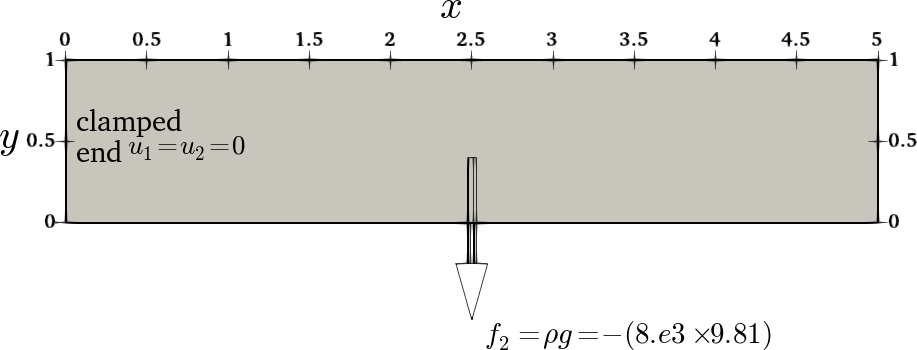
\includegraphics[width=0.5\textwidth]{./Images/le-2d-bar.png}
\caption{The 2D clamped bar problem. \label{2dbar-le-full}}
\end{figure}

\subsection{Step 1: Preprocessing}

First step in a PSD simulation is PSD preprocessing, at this step you
tell PSD what kind of physics, boundary conditions, approximations,
mesh, etc are you expecting to solve.

In the terminal \psd{cd} to the folder
\psd{/home/PSD-tutorials/linear-elasticity}
\footnote{Note that one can perform these simulation in any folder provided that PSD has been properly installed. We use \psd{/home/PSD-tutorials/linear-elasticity} for simplicity, once the user is proficient a simulation can be launch elsewhere.}.
Launch \psd{PSD\_PreProcess} from the terminal, to do so run the
following command.

\begin{lstlisting}[style=BashInputStyle]
PSD_PreProcess -problem linear_elasticity -dimension 2 -bodyforceconditions 1 \
-dirichletconditions 1 -postprocess u
\end{lstlisting}

After the \psd{PSD\_PreProcess} runs successfully you should see many
\psd{.edp} files in your current folder.

\textbf{What do the arguments mean ?}

\begin{itemize}
\item \psd{-problem linear\_elasticity} means that we are solving linear elasticity problem;
\item \psd{-dimension 2} means it is a 2D simulation;
\item \psd{-bodyforceconditions 1} with applied body force acting on the domain;
\item \psd{-dirichletconditions 1} says we have one Dirichlet border;
\item \psd{-postprocess u} means we would like to have ParaView post processing files.
\end{itemize}

At this stage the input properties \(E,\nu\) can be mentioned in
\psd{ControlParameters.edp}, use \psd{E = 200.e9}, and \psd{nu = 0.3;}.
The volumetric body force condition is mentioned in the same file via
variable \psd{Fbc0Fy -78480.0}, i.e (\(\rho*g=8.e3*(-9.81)=-78480.0\)).
One can also provide the mesh to be used in \psd{ControlParameters.edp},
via \psd{ThName = "../Meshes/2D/bar.msh"}
(\textit{note that mesh can also be provided in the next step}) .In
addition variable \psd{Fbc0On 1} has to be provided in order to indicate
the volume (region) for which the body force is acting, here \psd{1} is
the integer volume tag of the mesh. Dirichlet boundary conditions are
also provided in \psd{ControlParameters.edp}. To provide the clamped
boundary condition the variables \psd{Dbc0On 2}, \psd{Dbc0Ux 0.}, and
\psd{Dbc0Uy 0.} are used, which means for Dirichlet border \psd{2}
(\psd{Dbc0On 2}) where \psd{2} is the clamped border label of the mesh
Dirichlet constrain is applied and \psd{Dbc0Ux 0.}, \psd{Dbc0Uy 0} i.e.,
the clamped end condition (\(u_x=u_y=0\)).

\subsection{Step 2: Solving}

As PSD is a parallel solver, let us use 4 cores to solve the 2D bar
case. To do so enter the following command:

\begin{lstlisting}[style=BashInputStyle]
PSD_Solve -np 4 Main.edp -mesh ./../Meshes/2D/bar.msh -v 0
\end{lstlisting}

Here \psd{-np 4} denote the argument used to enter the number of
parallel processes (MPI processes) used while solving.
\psd{-mesh ./../Meshes/2D/bar.msh} is used to provide the mesh file to
the solver. \psd{-v 0} denotes the verbosity level on screen.
\psd{PSD\_Solve} is a wrapper around \psd{FreeFem++} or
\psd{FreeFem++-mpi}. Note that if your problem is large use more cores.
PSD has been tested upto 13,000 parallel processes and problem sizes
with billions of unknowns, surely you will now need that many for the 2D
bar problem.

\subsection{Step 3: Postprocessing}

PSD allows postprocessing of results in ParaView. After the step 2
mentioned above finishes. Launch ParaView and have a look at the
\psd{.pvd} file in the \psd{VTUs...} folder. Using ParaView for
postprocessing the results that are provided in the \psd{VTUs...}
folder, results such as those shown in
figure\textasciitilde{}\ref{bar-le-full} can be extracted.

\begin{figure}[h!]
\centering
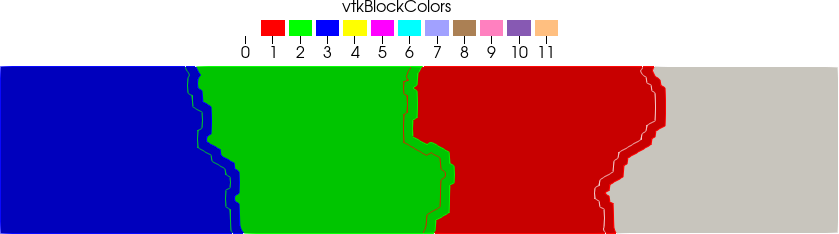
\includegraphics[width=0.4\textwidth]{./Images/le-2d-bar-partioned.png}\\
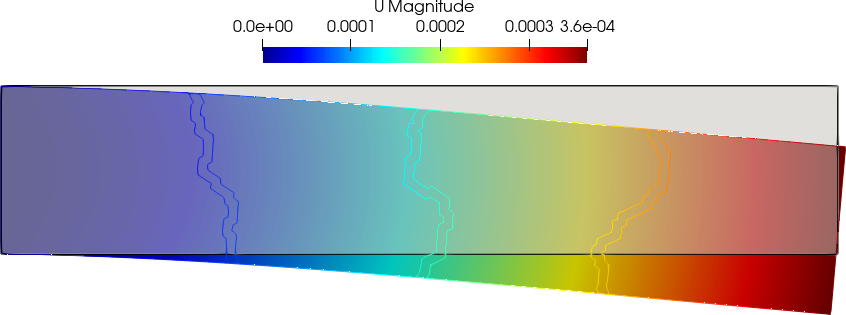
\includegraphics[width=0.4\textwidth]{./Images/le-2d-bar-results.png}
\caption{The 2D clamped bar problem: partitioned mesh and displacement field visualization in ParaView. \label{bar-le-full}}
\end{figure}

You are all done with your 2D linear-elasticty simulation.

\subsection{2D bar is ok, but what about 3D ?}

3D follows the same logic as 2D, in the preprocessing step

\begin{lstlisting}[style=BashInputStyle]
PSD_PreProcess -problem linear_elasticity -dimension 3 -bodyforceconditions 1 \
-dirichletconditions 1 -postprocess u
\end{lstlisting}

note that all what has changed \psd{-dimension 3} instead of
\psd{-dimension 2}

Solving step remains exactly the same with \psd{-mesh} flag now pointing
towards the \psd{3D} mesh.

\begin{lstlisting}[style=BashInputStyle]
PSD_Solve -np 4 Main.edp -mesh ./../Meshes/3D/bar.msh -v 0
\end{lstlisting}

\begin{figure}[h!]
\centering
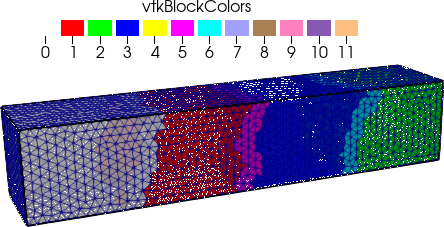
\includegraphics[width=0.4\textwidth]{./Images/le-3d-bar-clamped-ends.png}\\
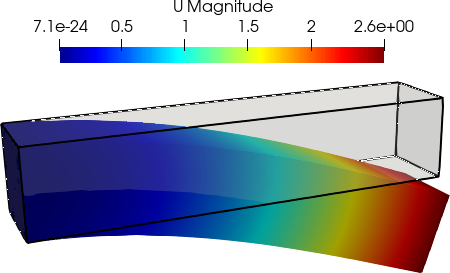
\includegraphics[width=0.4\textwidth]{./Images/le-3d-bar-clamped-pulled-partioned.png}
\caption{The 3D clamped bar problem: partitioned mesh and displacement field visualization in ParaView. \label{3dbar-le-full}}
\end{figure}

Using ParaView for postprocessing the results that are provided in the
\psd{VTUs...} folder, results such as those shown in
figure\textasciitilde{}\ref{3dbar-le-full} can be extracted.

}

\subsection{PSD simulation of of bar problem using a sequential solver (non parallel) \label{sec:2d-seq-load}}

{
	\renewcommand{\subsection}{\subsubsection}
	\newcommand{\psd}[1]{{\small\sffamily{\color{blue!60}#1}}}

Same problem of linear elasticity as in tutorial 1 -- 2D bar which bends
under its own load --, is discuss here. The bar 5 m in length and 1 m in
width, and is supposed to be made up of a material with density
\(\rho=8\times 10^3\), Youngs modulus \(E=200\times 10^9\), and Poissons
ratio \(\nu=0.3\). To avoid text repetition, readers are encouraged to
go ahead with this tutorial only after tutorial 1.

As we will not use a parallel solver but a sequential one, naturally,
this tutorial leads to a slow solver than the previous tutorial 1. So
this tutorial is not for speed lovers, but rather for detailing the full
capacity of PSD. Also sequential solvers are easier to develop and
understand hence this tutorial.

As the problem remains same as tutorial 1, simply add \psd{-sequential}
flag to \psd{PSD\_PreProcess} flags from tutorial 1 for a PSD sequential
solver. The flag \psd{-sequential} signifies the use of sequential PSD
solver. So the work flow for the 2D problem would be:

\begin{lstlisting}[style=BashInputStyle]
PSD_PreProcess -problem linear_elasticity -dimension 2 -bodyforceconditions 1 \
-dirichletconditions 1 -postprocess u -sequential
\end{lstlisting}

Similar to tutorial 1, We solve the problem using the given mesh file
\psd{bar.msh}. However now we need to use \psd{PSD\_Solve\_Seq} instead
of \psd{PSD\_Solve}, as such:

\begin{lstlisting}[style=BashInputStyle]
PSD_Solve_Seq Main.edp -mesh ./../Meshes/2D/bar.msh -v 0
\end{lstlisting}

Users are encouraged to try out the 3D problem with sequential solver.
Also comparing the results from a sequential solver to that form a
parallel solver can be verified to assure that the both parallel and
sequential solvers lead to exactly the same results.

Note that for this simple problem, the bar mesh (\psd{bar.msh}) has been
provided in \psd{../Meshes/2D/"} folder, this mesh is a triangular mesh
produced with Gmsh. Moreover detailing meshing procedure is not the
propose of PSD tutorials. A user has the choice of performing their own
meshing step and providing them to PSD in
\psd{.msh}\footnote{Please use version 2} or \psd{.mesh} format, we
recommend using Salome or Gmsh meshers for creating your own geometry
and meshing them.

\subsection{Comparing CPU time}

Naturally, since we are not using parallel PSD for solving, we lose the
advantage of solving fast. To testify this claim checking solver timings
can be helpful. PSD provides means to time log your solver via
\psd{-timelog} flag. What this will do when you run your solver, on the
terminal you will have information printed on what is the amount of time
taken by each step of your solver. Warning, this will make your solver
slower, as this action involves `MPI\_Barrier' routines for correctly
timing operation.

An example work flow of 2D solver (parallel) with timelogging:

\begin{lstlisting}[style=BashInputStyle]
PSD_PreProcess -problem linear_elasticity -dimension 2 -bodyforceconditions 1 \
-dirichletconditions 1 -postprocess u -timelog
\end{lstlisting}

We solve the problem using four MPI processes, with the given mesh file
\psd{bar.msh}.

\begin{lstlisting}[style=BashInputStyle]
PSD_Solve -np 4 Main.edp -mesh ./../Meshes/2D/bar.msh -v 0
\end{lstlisting}

\begin{figure}[h!]
\centering
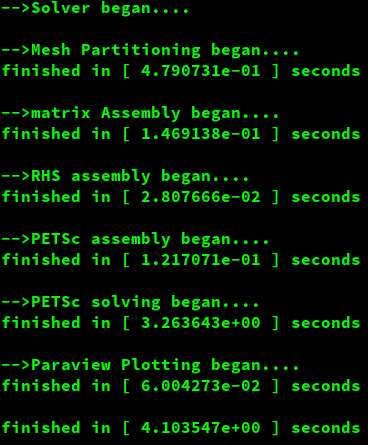
\includegraphics[width=0.4\textwidth]{./Images/le-time-par.png}
\caption{Time logging output produced for parallel run on 4 processes.\label{time-par-le}}
\end{figure}

The \cref{time-par-le} shows the time logging output produced for
parallel run on 4 processes using \psd{-timelog} flag. Take note of
timings produced for different operations of the solver.

Now let us repeat the procedure but this time use sequential solver:

\begin{lstlisting}[style=BashInputStyle]
PSD_PreProcess -problem linear_elasticity -dimension 2 -bodyforceconditions 1 \
-dirichletconditions 1 -postprocess u -timelog -sequential
\end{lstlisting}

We solve the problem now in sequential, with the given mesh file
\psd{bar.msh}.

\begin{lstlisting}[style=BashInputStyle]
PSD_Solve_Seq Main.edp -mesh ./../Meshes/2D/bar.msh -v 0
\end{lstlisting}

You should now see timings that are higher in comparison to the parallel
solver. Approximately, for large meshes using 4 MPI processes should
lead to 4 times fast solver.

}



\subsection{PSD simulation of 2D bar problem clamped at both ends \label{sec:2D-bar-clamped1}}

{
	\renewcommand{\subsection}{\subsubsection}
	\newcommand{\psd}[1]{{\small\sffamily{\color{blue!60}#1}}}


To showcase the usage of Linear elasticity, we shall discuss here an
example of a 2D bar, which bends under its own load. The bar
\(5\times1\) m\(^2\) in area is made up of material with
\(\rho=8\times 10^3\), \(E=200\times 10^9\), and \(\nu=0.3\). Contrary
to tutorial 1, now both ends of the bar are clamped.

\subsection{Step 1: Preprocessing}

First step in a PSD simulation is PSD preprocessing , at this step you
tell PSD what kind of physics, boundary conditions, approximations,
mesh, etc are you expecting to solve.

In the terminal \psd{cd} to the folder
\psd{/home/PSD-tutorials/linear-elasticity}. Launch
\psd{PSD\_PreProcess} from the terminal, to do so run the following
command.

\begin{lstlisting}[style=BashInputStyle]
PSD_PreProcess -problem linear_elasticity -dimension 2 -bodyforceconditions 1 \
-dirichletconditions 2 -postprocess u
\end{lstlisting}

After the \psd{PSD\_PreProcess} runs successfully you should see many
\psd{.edp} files in your current folder.

\textbf{What do the arguments mean ?}

\begin{itemize}
\item \psd{-problem linear\_elasticity} means that we are solving linear elasticity problem;
\item \psd{-dimension 2} means it is a 2D simulation;
\item \psd{-bodyforceconditions 1} with applied body force acting on the domain;
\item \psd{-dirichletconditions 2} says we have two Dirichlet border;
\item \psd{-postprocess u} means we would like to have ParaView post processing files.

\end{itemize}

Since basic nature of both the problems (the one from tutorial 1 and 2)
is same the almost the same command for preprocessing used in previous
tutorial 1 is used here. The only difference,is that an additional
Dirichlet condition needs to be supplied, notified to PSD by
\psd{ -dirichletconditions 2}. To provide Dirichlet conditions of the
left clamped end (\(u_x=u_y=0\)) in \psd{ControlParameters.edp} set
\psd{Dbc0On 2}, \psd{Dbc0Ux 0.}, and \psd{Dbc0Uy 0.}. Similarly, for the
right end set variables \psd{Dbc1On 4}, \psd{Dbc1Ux 0.}, and
\psd{Dbc1Uy 0}. Each one of these is a clamped border respectively
labeled as 2 (\psd{Dbc0On 2}) and 4 (\psd{Dbc1On 4}) in the mesh
\psd{../Meshes/2D/bar.msh}.

Just like the previous tutorial the input properties \(E,\nu\) should be
mentioned in \psd{ControlParameters.edp}, use \psd{E = 200.e9}, and
\psd{nu = 0.3;}. The volumetric body force condition is mentioned in the
same file via variable \psd{Fbc0Fy -78480.0}, i.e
(\(\rho*g=8.e3*(-9.81)=-78480.0\)). One can also provide the mesh to be
used in \psd{ControlParameters.edp} , via
\psd{ThName = "../Meshes/2D/bar.msh"}
(\textit{note that mesh can also be provided in the next step}) .In
addition variable \psd{Fbc0On 1} has to be provided in order to indicate
the volume (region) for which the body force is acting, here \psd{1} is
the integer volume tag of the mesh.

\subsection{Step 2: Solving}

As PSD is a parallel solver, let us use 3 parallel processes to solve
this 2D bar case. To do so enter the following command:

\begin{lstlisting}[style=BashInputStyle]
PSD_Solve -np 3 Main.edp -mesh ./../Meshes/2D/bar.msh -v 0
\end{lstlisting}

Here \psd{-np 3} denote the argument used to enter the number of
parallel processes (MPI processes) used while solving.
\psd{-mesh ./../Meshes/2D/bar.msh} is used to provide the mesh file to
the solver. \psd{-v 0} denotes the verbosity level on
screen.\psd{PSD\_Solve} is a wrapper around \psd{FreeFem++} or
\psd{FreeFem++-mpi}. Note that if your problem is large use more cores.
PSD has been tested upto 13,000 parallel processes and problem sizes
with billions of unknowns, surely you will now need that many for the 2D
bar problem.

\subsection{Step 3: Postprocessing}

PSD allows postprocessing of results in ParaView. After the step 2
mentioned above finishes. Launch ParaView and have a look at the
\psd{.pvd} file in the \psd{VTUs\_DATE\_TIME} folder. Using ParaView for
postprocessing the results that are provided in the \psd{VTUs...}
folder, results such as those shown in
figure\textasciitilde{}\ref{bar-le-full-n} can be extracted.

\begin{figure}[h!]
\centering
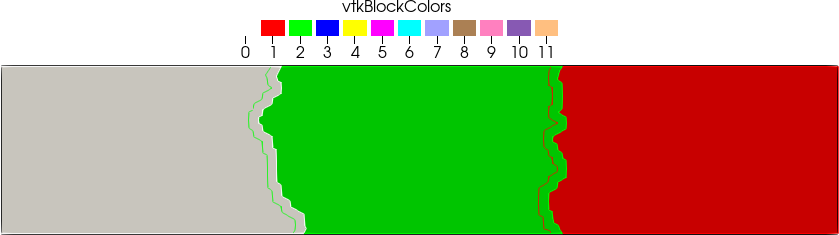
\includegraphics[align=t,width=0.4\textwidth]{./Images/le-2d-bar-partitioned3.png}\hfill
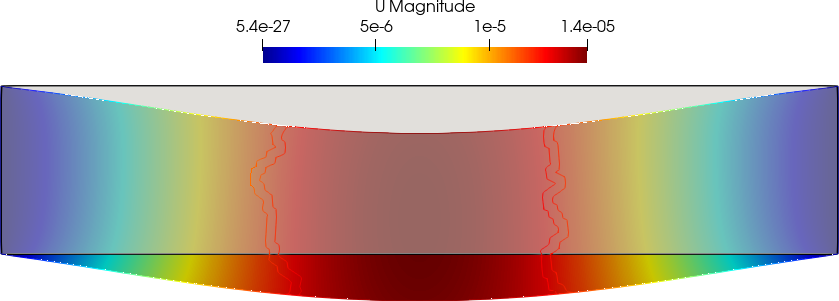
\includegraphics[align=t,width=0.4\textwidth]{./Images/le-2d-bar-clamped-ends.png}
\caption{The 2D clamped bar problem: partitioned mesh and displacement field visualization in ParaView. \label{bar-le-full-n}}
\end{figure}

You are all done with your 2D linear-elasticity simulation.

Try running the 3D problem. Keep in mind to rerun the
\psd{PSD\_PreProcess} with \psd{-dimension 3} flag and using the
appropriate mesh via \psd{-mesh} flag with \psd{PSD\_Solve}. It goes
without saying you will need to adjust the Dirichlet border labels in
\psd{ControlParameters.edp}.

\subsection{Redoing the test on Jupiter and moon}

Imagine, you wish to know how the test would compare if performed on
Moon and Jupiter. Since gravity is the main force involved in the
problem, try redoing the test with different gravitational constant. The
only thing that will change now is the gravitational pull, for Moon
\(g=1.32\) and for Jupiter \(g=24.79\). To perform the moon test simply
change \psd{Fbc0Fy -10560.0} in \psd{ControlParameters.edp} and redo
step 2 and step 3. Similarly, for the Jupiter test
\psd{Fbc0Fy -198320.0} in \psd{ControlParameters.edp} and redo step 2
and step 3.

\begin{figure}[htbp]
    \centering
    \begin{minipage}[t][2.5cm][t]{0.4\textwidth}
    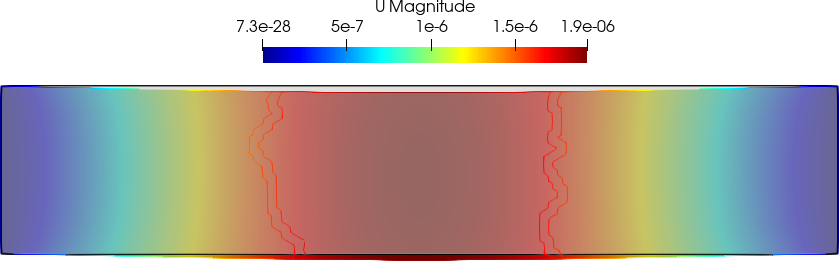
\includegraphics[align=t,width=1\textwidth]{./Images/le-2d-bar-moon.png}
    \end{minipage}\hspace{.1\textwidth}
    \begin{minipage}[t][2.5cm][t]{0.4\textwidth}
    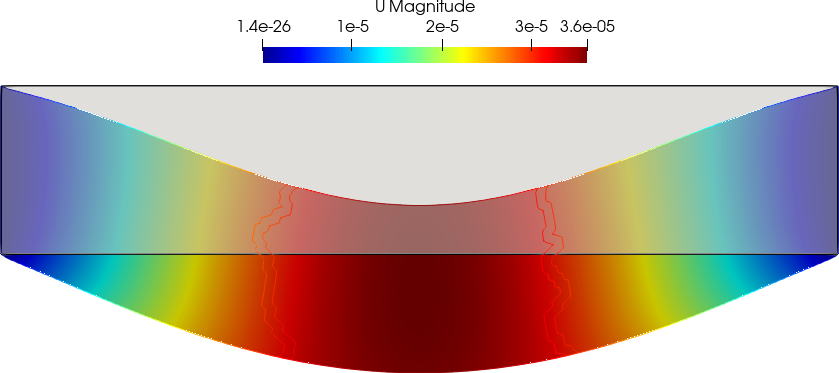
\includegraphics[align=t,width=1\textwidth]{./Images/le-2d-bar-Jupiter.png}
    \end{minipage}
    \caption{2D clamped bar 20000X warped displacement fields. On moon (left) and  on Jupiter (right).}
    \label{fig:moon-jupiter}
\end{figure}

}


\subsection{PSD simulation of 2D bar problem clamped at one end wile being pulled at the other end (Dirichlet-Dirichlet case)\label{sec:2d-bar-clamped2}}

{
	\renewcommand{\subsection}{\subsubsection}
	\newcommand{\psd}[1]{{\small\sffamily{\color{blue!60}#1}}}

We reintroduce the problem from tutorial 1, an example of a 2D bar which
bends under its own load -- typical case of linear elasticity. The bar
\(5\times1\) m\(^2\) in area is made up of material with
\(\rho=8\times 10^3\), \(E=200\times 10^9\), and \(\nu=0.3\).

\begin{figure}[h!]
\centering
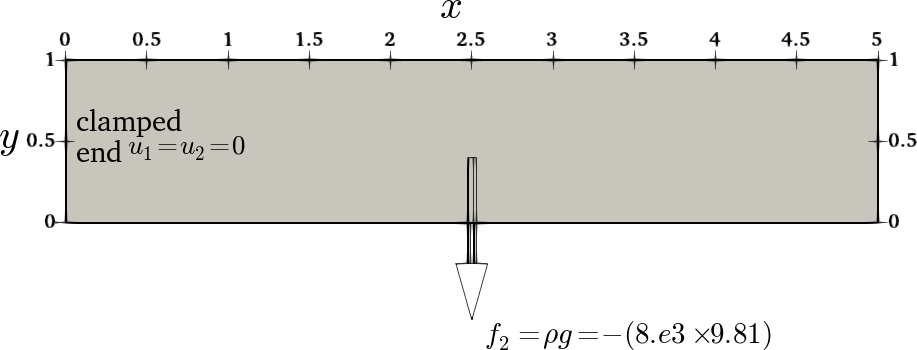
\includegraphics[width=0.5\textwidth]{./Images/le-2d-bar.png}
\caption{The 2D clamped bar problem. \label{2dbar-le-full}}
\end{figure}

\subsection{Step 1: Preprocessing}

First step in a PSD simulation is PSD preprocessing, at this step you
tell PSD what kind of physics, boundary conditions, approximations,
mesh, etc are you expecting to solve. More importantly for this tutorial
we will signify to PSD that MFront has to be used.

In the terminal \psd{cd} to the folder
\psd{/home/PSD-tutorials/linear-elasticity}. Launch
\psd{PSD\_PreProcess} from the terminal, to do so run the following
command.

\begin{lstlisting}[style=BashInputStyle]
PSD_PreProcess -problem linear_elasticity -dimension 2 -bodyforceconditions 1 \
-dirichletconditions 1 -postprocess u -useMfront
\end{lstlisting}

After the \psd{PSD\_PreProcess} runs successfully you should see many
\psd{.edp} files in your current folder.

\textbf{What do the arguments mean ?}

\begin{itemize}
\item \psd{-problem linear\_elasticity} means that we are solving linear elasticity problem;
\item \psd{-dimension 2} means it is a 2D simulation;
\item \psd{-bodyforceconditions 1} with applied body force acting on the domain;
\item \psd{-dirichletconditions 1} says we have one Dirichlet border;
\item \psd{-postprocess u} means we would like to have ParaView post processing files.
\item \psd{-useMfront} activates MFront interface for PSD.
\end{itemize}

At this stage the input properties \(E,\nu\) can be mentioned in
\psd{ControlParameters.edp}, use \psd{E = 200.e9}, and \psd{nu = 0.3}.
In contrast to tutorial 1, notice that these values of \psd{E} and
\psd{nu} are fed to a vector \psd{PropertyValues = [E, nu];} verbosed by
\psd{PropertyNames   = "YoungModulus PoissonRatio";}. We also signify
that we will be solving linear elasticity via
\psd{MforntMaterialBehaviour   = "Elasticity";} and also
\psd{MaterialHypothesis = "GENERALISEDPLANESTRAIN";} which signifies the
hypothesis to be used for the Linear elasticity
\footnote{The \psd{MaterialHypothesis} accepts \psd{"GENERALISEDPLANESTRAIN"},  \psd{"PLANESTRAIN"}, \psd{"PLANESTRESS"},  and  \psd{"TRIDIMENSIONAL"} as arguments.}.
\psd{PropertyValues}, \psd{PropertyNames}, and \psd{MaterialHypothesis}
will eventually be provided to MFront in \psd{FemParameters.edp} file
via \psd{mfrontElasticityHandler(...)} function
\footnote{User is encouraged to have a look at \psd{FemParameters.edp} file.}.
The volumetric body force condition is mentioned in the same file via
variable \psd{Fbc0Fy -78480.0}, i.e (\(\rho*g=8.e3*(-9.81)=-78480.0\)).
One can also provide the mesh to be used in \psd{ControlParameters.edp},
via \psd{ThName = "../Meshes/2D/bar.msh"}
(\textit{note that mesh can also be provided in the next step}) .In
addition variable \psd{Fbc0On 1} has to be provided in order to indicate
the volume (region) for which the body force is acting, here \psd{1} is
the integer volume tag of the mesh. Dirichlet boundary conditions are
also provided in \psd{ControlParameters.edp}. To provide the clamped
boundary condition the variables \psd{Dbc0On 2}, \psd{Dbc0Ux 0.}, and
\psd{Dbc0Uy 0.} are used, which means for Dirichlet border \psd{2}
(\psd{Dbc0On 2}) where \psd{2} is the clamped border label of the mesh
Dirichlet constrain is applied and \psd{Dbc0Ux 0.}, \psd{Dbc0Uy 0} i.e.,
the clamped end condition (\(u_x=u_y=0\)).

\subsection{Step 2: Solving}

As PSD is a parallel solver, let us use 4 cores to solve the 2D bar
case. To do so enter the following command:

\begin{lstlisting}[style=BashInputStyle]
PSD_Solve -np 4 Main.edp -mesh ./../Meshes/2D/bar.msh -v 0
\end{lstlisting}

Here \psd{-np 4} denote the argument used to enter the number of
parallel processes (MPI processes) used while solving.
\psd{-mesh ./../Meshes/2D/bar.msh} is used to provide the mesh file to
the solver. \psd{-v 0} denotes the verbosity level on screen.
\psd{PSD\_Solve} is a wrapper around \psd{FreeFem++} or
\psd{FreeFem++-mpi}. Note that if your problem is large use more cores.
PSD has been tested upto 13,000 parallel processes and problem sizes
with billions of unknowns, surely you will now need that many for the 2D
bar problem.

\subsection{Step 3: Postprocessing}

PSD allows postprocessing of results in ParaView. After the step 2
mentioned above finishes. Launch ParaView and have a look at the
\psd{.pvd} file in the \psd{VTUs...} folder. Using ParaView for
postprocessing the results that are provided in the \psd{VTUs...}
folder, results such as those shown in
figure\textasciitilde{}\ref{bar-le-full} can be extracted.

\begin{figure}[h!]
\centering
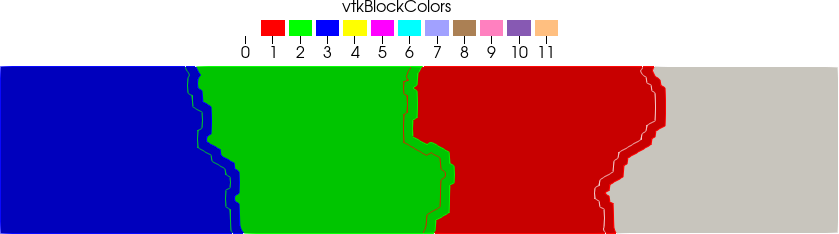
\includegraphics[width=0.4\textwidth]{./Images/le-2d-bar-partioned.png}\\
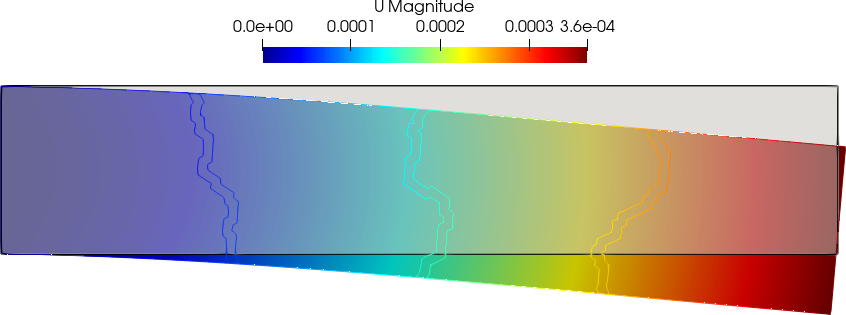
\includegraphics[width=0.4\textwidth]{./Images/le-2d-bar-results.png}
\caption{The 2D clamped bar problem: partitioned mesh and displacement field visualization in ParaView. \label{bar-le-full}}
\end{figure}

You are all done with your 2D linear-elasticty simulation with Mfront
interface.

\subsection{How and what is being done in PSD-MFront interface? }

To explain how PSD-MFront interface works we will compare how a PSD
solver acts when using MFront or without. In other words what is
different when \psd{-useMfront} is used at preprocessing. Note that
ultimately the problem results (displacement fields, stresses, strains)
will be the same.

To put it briefly, what MFront does for linear elasticity problem here
is build the Material tensor (stiffness matrix) at each quadrature
point. So, there are two points

\begin{itemize}
\item We need to communicate to Mfront the nature of the problem and the material involved.
\item We need to provide Mfornt the stiffness matrix at each quadrature point so that it can fill it up.
\end{itemize}

The two raised points are handled using
\psd{mfrontElasticityHandler(...)} in \psd{FemParameters.edp} file.

Firstly, the arguments \psd{E = 200.e9}, \psd{nu = 0.3},
\psd{MforntMaterialBehaviour   = "Elasticity";},
\psd{PropertyValues = [E, nu];},
\psd{PropertyNames   = "YoungModulus PoissonRatio";},
\psd{PropertyValues = [E, nu];} and
\psd{MaterialHypothesis = "GENERALISEDPLANESTRAIN";} form
\psd{ControlParameters.edp} takes care of the first point (the nature of
the problem and the material involved). The latter three arguments well
define that we have a 2D problem, with given values of properties
(\(E, \nu\)). The snippet from \psd{ControlParameters.edp} (produced
after using \psd{-useMfront} argument for \psd{PSD\_PreProcess}) file
shows these variables which define the nature of the problem and
characteristics of material involved

\begin{lstlisting}[style=CppStyle]
//============================================================================
//                   ------- Material parameters -------
// -------------------------------------------------------------------
//  E, nu : Modulus of Elasticity and Poisson ratio of the material
//  PropertyNames : String of material property names (space seperated)
//                  that are provided to Mfront.
//  PropertyValues : Values of material properties provided to Mfront
//
// -------------------------------------------------------------------
//  NOTE:     Please note that PropertyNames should be the same as
//            as in the Elasticity.mfront file
// -------------------------------------------------------------------
//============================================================================

  macro E()  200.e9  //
  macro nu() 0.3     //

  string    MaterialBehaviour  = "Elasticity";
  string    MaterialHypothesis = "GENERALISEDPLANESTRAIN";
  string    PropertyNames      = "YoungModulus PoissonRatio";
  real[int] PropertyValues     = [ E, nu ];
\end{lstlisting}

Secondly, the to get the stiffness matrix from Mfornt we use a
quadrature finite element space with vector finite elements built on it
(6 components) that represent the 6 components of symmetric material
tensor (\(\mathbb R^{3 \times 3}\)). The snippet from
\psd{MeshAndFeSpace.edp} file shows the 6 component Quadrature finite
element space for building material tensor.

\begin{lstlisting}[style=CppStyle]
//==============================================================================
// ------- The finite element space  -------
// ----------------------------------------------------------------------------
//  Qh       : Quadratur finite element space  for material tensor
//             FEQF2 implies 3 dof for a triangular cell in the mesh
//             A vectorial FEM space is built with 6 components
//==============================================================================

 fespace Qh  ( Th ,[ FEQF2, FEQF2, FEQF2,
                           FEQF2, FEQF2,
                                  FEQF2] );
\end{lstlisting}

Finally in file \psd{FemParameters.edp} the
\psd{mfrontElasticityHandler()} is called to build the material tensor
\psd{Mt} provided with the previously built material properties and
nature of problem. Please see the snippet below

\begin{lstlisting}[style=CppStyle]
//============================================================================
// ------- Material Tensor using Quadrature FE space -------
// -------------------------------------------------------------------
// Mt[int]  : is an array of finite element variable belonging to quadratu
//            re space Qh. This array is used  to define components of the
//            material tensor. 3X3 in 2D and 6X6 in 3D
//            In 2D the material tensor looks like
//
//         [ 2*mu+lambda ,  lambda      , 0 ]    [ Mt11 , Mt12 , Mt13 ]
//   Mt =  [ lambda      ,  2*mu+lambda , 0 ] =  [ Mt12 , Mt22 , Mt23 ]
//         [   0         ,     0        , mu]    [ Mt13 , Mt23 , Mt33 ]
//
// mfrontElasticityHandler : is a function in mfront interface that helps
//                           building the material tensor  Mt  given with
//                           material prpts.  from  ControlParameters.edp
//============================================================================

  Qh [ Mt11 ,  Mt12 , Mt13 ,
              Mt22 , Mt23 ,
                     Mt33 ];


  mfrontElasticityHandler( MforntMaterialBehaviour                             ,
                           mfrontBehaviourHypothesis = MaterialHypothesis      ,
                           mfrontPropertyNames       = PropertyNames           ,
                           mfrontPropertyValues      = PropertyValues          ,
                           mfrontMaterialTensor      = Mt11[]
                         );
\end{lstlisting}

Note that in the snippet above you might be seeing \psd{Mt11[]} being
provided as \psd{mfrontMaterialTensor}, in fact the \psd{Mt11[]} calls
the full matrial tensor not just the first component, so user should not
get confused
\footnote{This is more technical note, \psd{Mt11[]} is the cast of \psd{Mt} vector to a single array for memory optimization. One can also simply use \psd{Mt12[]}, \psd{Mt13[]}, \psd{Mt22[]}, ... all these are acceptable and are simply aliases to material tensor.}.

The material tensor \psd{Mt} built is used in the finite element
variational formulation to build the bilinear
\(a(\mathbf{u},\mathbf{v})\) which is used to assemble the finite
element matrix \(\mathbf{A}\) for the linear system
\(\mathbf{Ax} = \mathbf{b}\)

\[
a(\mathbf{u},\mathbf{v}) = \int_{\Omega}(
                 \varepsilon \left(\mathbf{u}):\mathbf{Mt}:\varepsilon(\mathbf{v}\right)
               )
\]

Here, \(\mathbf{u}:\mathbf{Mt}\) is nothing but the stress
\(\sigma(\mathbf{u})\) operator. User is encourage to have a look at the
\psd{VariationalFormulation.edp} file that contains the variational
formulation (weak form) of the problem described.

}



\subsection{PSD simulation of 2D bar problem clamped at one end wile being pulled at the other end (Dirichlet--Neumann case)\label{sec:2d-bar-clamped3}}

{
	\renewcommand{\subsection}{\subsubsection}
	\newcommand{\psd}[1]{{\small\sffamily{\color{blue!60}#1}}}

Similar simulation, as in the prvious tutorial is presented in this
section. We showcase the 2D bar problem simulation with one end clamped
wile being pulled at the other end. Just like the previous simulation
the body force is neglected, However now the non clamped ends pull is
approximated with Neumann force
\(\int_{\partial\Omega^h_{\text N}}(\mathbf t \cdot \mathbf{v}^h)\). To
simulate the pull we assume traction vector
\(\mathbf t=[t_x,t_y]=[10^9.,0]\) acting on the non clamped right end of
the bar, i.e., force in \(x\) direction is 10 units. Here is how PSD
simulation of this case can be performed.

\textbf{Step 1: Preprocessing}

For ``PSD preprocessing'' go to any folder, launch the terminal there
and run the following command.

\begin{lstlisting}[style=BashInputStyle]
PSD_PreProcess -problem linear-elasticity -dimension 2 -dirichletconditions 1 -tractionconditions 1 -postprocess u
\end{lstlisting}

the comandline flag \psd{ -dirichletconditions 1}, notifies to PSD that
there is one Dirichlet border ---the clamped end of the bar--- in this
simulation. And the flag \psd{ -tractionconditions 1} notifies to PSD
that there is one traction border ---the right end of the bar--- in this
simulation. To provide the clamped boundary condition (\(u_1=0,u_2=0\))
set the variables \psd{ Dbc0On 2}, \psd{ Dbc0Ux 0.}, and
\psd{ Dbc0Uy 0.} in \psd{ ControlParameters.edp}. In the same file
traction boundary conditions are provided via the variables
\psd{ Tbc0On 4} and \psd{ Tbc0Tx 1.e9}, which mean apply traction force
\(\mathbf t=[t_x,t_y]=[10^9.,0]\) on label number 4 (right) of the mesh.
If user wishes to add traction force ,for instance \(t_y=100.\), simply
add the missing macro \psd{ macro Tbc0Tx 1.e9 //}.

\textbf{Step 2: Solving}

Let us now use 5 cores to solve this problem. To do so enter the
following command:

\begin{lstlisting}[style=BashInputStyle]
PSD_Solve -np 5 Main.edp
\end{lstlisting}

Notice, that this is the exact same command used in solving the previous
bar problems from other sections, with only difference that we now use
\psd{ -np 5}.

\textbf{Step 3: Postprocessing}

Launch ParaView and have a look at the \psd{ .pvd} file in the
\psd{ PSD/Solver/VTUs\_DATE\_TIME} folder.

\begin{figure}[htbp]
    \centering
    \begin{minipage}[t][2cm][t]{0.36\textwidth}
    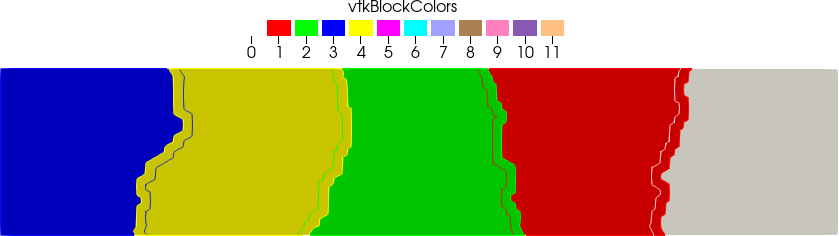
\includegraphics[align=b,width=1\textwidth]{./Images/2d-bar-partitioned5.png}
    \end{minipage}\hspace{.1\textwidth}
    \begin{minipage}[t][2cm][t]{0.5\textwidth}
    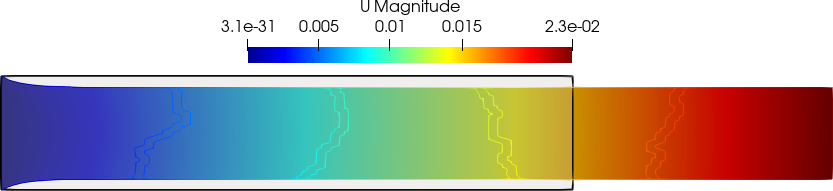
\includegraphics[align=b,width=1\textwidth]{./Images/2d-bar-clamped-traction.png}
    \end{minipage}
    \caption{2D bar results. Partitioned mesh (left) and 100X warped displacement field (right).}
    \label{fig:5part}
\end{figure}

Note now in\textasciitilde{}\ref{fig:5part} there are five subdomains in
the partitioned mesh since five cores were used. Contrary to previous
tutorial, as expected, we see that the right end of the bar which is
being pulled now contract in \(y\) direction. This is due to the fact
that there is no Dirichlet condition at this end now.

}
 

\subsection{PSD simulation of 2D bar problem clamped at one end wile being pulled at the other end (Dirichlet-Neumann-Point boundary conditions case)\label{sec:2d-bar-clamped4}}


{
	\renewcommand{\subsection}{\subsubsection}
	\newcommand{\psd}[1]{{\small\sffamily{\color{blue!60}#1}}}

Similar simulations, as in the prvious tutorial is presented in this
section. We showcase the 2D bar problem simulation with one end clamped
wile being pulled at the other end. Contrary to simulation in the
previous tutorial, the clamped end just restricts \(x\) movement, i.e,
\(u_x=0\). Just like simulation from the prvious tutorial the body force
is neglected. Just like simulation in the prvious tutorial , the non
clamped ends pull is approximated with Neumann force
\(\int_{\partial\Omega^h_{\text N}}(\mathbf t\cdot \mathbf{v}^h)\). To
simulate the pull we assume traction vector
\(\mathbf t=[t_x,t_y]=[10^9,0]\) acting on the non clamped right end of
the bar, i.e., force in \(x\) direction is \(10^9\) units. Here is how
PSD simulation of this case can be performed.

\textbf{Step 1: Preprocessing}

For ``PSD preprocessing'' go to any folder, launch the terminal there
and run the following command.

\begin{lstlisting}[style=BashInputStyle]
PSD_PreProcess -problem linear-elasticity -dimension 2 -dirichletconditions 1 -tractionconditions 1 \
-dirichletpointconditions 1 -postprocess u
\end{lstlisting}

Additional flag \psd{ -dirichletpointconditions 1} now appears, this
notifies to PSD that there is one Dirichlet point boundary condition.
Edit the \psd{ ControlParameters.edp} to communicate the desired point
boundary conditions, set the variables \psd{ Pbc0Ux  0.} and
\psd{ Pbc0Uy  0.} to specify \(u_x=0,u_y=0\), and variable
\psd{ PbcCord = [[  0. , 0. ]];} to specify the point coordinates
\((x,y)=(0,0)\). Via the flags we specified that
\psd{ -dirichletconditions 1}, i.e., there is one Dirichlet border. To
provide the Dirichlet condition (\(u_x=0\)) set the variables
\psd{ Dbc0On 2} and \psd{ Dbc0Ux 0.} in \psd{ ControlParameters.edp}.
PSD understands that 4 is the mesh border label on which Dirichlet is
applied and (\(u_x=0\)) is the condition to be applied.

\textbf{Step 2: Solving}

Let us now use 6 cores to solve this problem. To do so enter the
following command:

\begin{lstlisting}[style=BashInputStyle]
PSD_Solve -np 6 Main.edp
\end{lstlisting}

\% Notice, that this is the exact same command used in solving the
previous bar problems from other sections, with only difference that we
now use \psd{ -np 6}.

\textbf{Step 3: Postprocessing}

Launch ParaView and have a look at the \psd{ .pvd} file in the
\psd{ PSD/Solver/VTUs\_DATE\_TIME} folder.

\begin{figure}[htbp]
    \centering
    \begin{minipage}[t][2cm][t]{0.36\textwidth}
    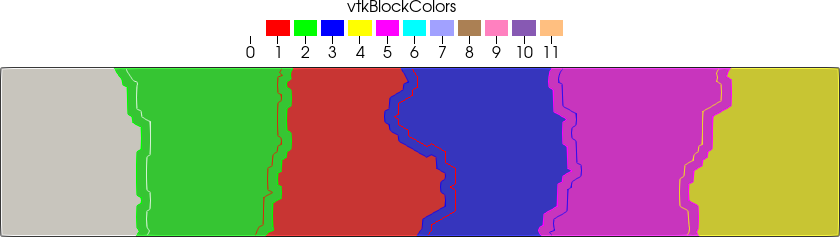
\includegraphics[align=b,width=1\textwidth]{./Images/2d-bar-partitioned6.png}
    \end{minipage}\hspace{.1\textwidth}
    \begin{minipage}[t][2cm][t]{0.5\textwidth}
    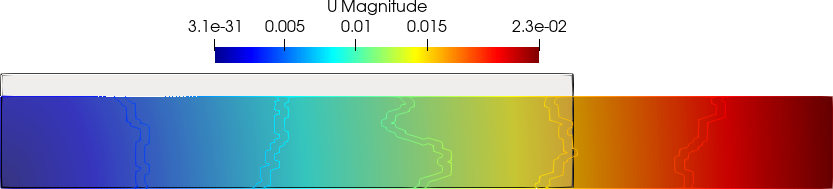
\includegraphics[align=b,width=1\textwidth]{./Images/2d-bar-clamped-traction-point.png}
    \end{minipage}
    \caption{2D bar results. Partitioned mesh (left) and 100X warped displacement field (right).}
    \label{fig:6part}
\end{figure}

Note now in\textasciitilde{}\cref{fig:6part} there are six subdomais in
the partitioned mesh. As expected, we see that the right and the left
end of the bar which is being pulled now contract in \(y\) direction,
and the bar elongates in \(x\) direction.

}


\subsection{PSD simulation of 3D bar problem clamped at one end wile being pulled at the other end (Dirichlet-Neumann case)\label{sec:3d-bar-clamped3}}

{
	\renewcommand{\subsection}{\subsubsection}
	\newcommand{\psd}[1]{{\small\sffamily{\color{blue!60}#1}}}

In this section we present a 3D PSD simulation of a clamped bar which
his being loaded in vertical direction at the non-clamped end. This
simulation is like the one presented in previous tutorials, however in
3D. The material properties are same as before, and at the non-clamped
end traction \(t_y=-10^9\) units.The same problem from previous
tutorials 1 and 2 is used here in 3D, a bar 5 m in length and 1 m in
width and 1 m in height, and is supposed to be made up of a material
with density \(\rho=8\times 10^3\), Youngs modulus \(E=200\times 10^9\),
and Poissons ratio \(\nu=0.3\).

Here is how PSD simulation of this case can be performed.

\textbf{Step 1: Preprocessing}

First step in a PSD simulation is PSD preprocessing, at this step you
tell PSD what kind of physics, boundary conditions, approximations,
mesh, etc are you expecting to solve.

In the terminal \psd{cd} to the folder
\psd{/home/PSD-tutorials/linear-elasticity}. Launch
\psd{PSD\_PreProcess} from the terminal, to do so run the following
command.

\begin{lstlisting}[style=BashInputStyle]
PSD_PreProcess  -problem linear-elasticity -dimension 3 -dirichletconditions 1 -tractionconditions 1 -postprocess u
\end{lstlisting}

the comandline flag \psd{ -dirichletconditions 1} notifies to PSD that
there is one Dirichlet border ---the clamped end of the bar--- in this
simulation; \psd{ -dimension 3} means the simulation is 3D. And the flag
\psd{ -tractionconditions 1} notifies to PSD that there is one traction
border ---the right end of the bar--- in this simulation.

To provide Dirichlet conditions of the clamped end
(\(u_x=0,u_y=0,u_z=0\)) in \psd{ ControlParameters.edp} set
\psd{ Dbc0On 1}, \psd{ Dbc0Ux 0.}, \psd{ Dbc0Uy 0.}, and
\psd{ Dbc0Uz 0.}, where 1 being the surface mesh label of the clamped
end. To add the traction boundary condition set \psd{ Tbc0On 2} and
\psd{ Tbc0Ty -1.e9}, here the mesh label number of the right end is 2.
For this end \(\mathbf t=[t_x,t_y,t_z]=[0.,10^9,0.]\), hence in
\psd{ ControlParameters.edp} we only use \psd{ Tbc0Ty -1.e9}.

\textbf{Step 2: Solving}

Let us now use 4 cores to solve this problem. To do so enter the
following command:

\begin{lstlisting}[style=BashInputStyle]
PSD_Solve -np 4 Main.edp  -mesh ./../Meshes/3D/bar.msh -v 0
\end{lstlisting}

Notice, that this is the exact same command used in solving the previous
bar problems from other tutorials.

Note that for this simple problem, the bar mesh (\psd{bar.msh}) has been
provided in \psd{../Meshes/3D/"} folder, this mesh is a triangular mesh
produced with Gmsh. Moreover detailing meshing procedure is not the
propose of PSD tutorials. A user has the choice of performing their own
meshing step and providing them to PSD in
\psd{.msh}\footnote{Please use version 2} or \psd{.mesh} format, we
recommend using Salome or Gmsh meshers for creating your own geometry
and meshing them.

\textbf{Step 3: Postprocessing}

Launch ParaView and have a look at the \psd{ .pvd} file in the
\psd{ PSD/Solver/VTUs\_DATE\_TIME} folder.

\begin{figure}[htbp]
    \centering
    \begin{minipage}[t][2cm][t]{0.38\textwidth}
    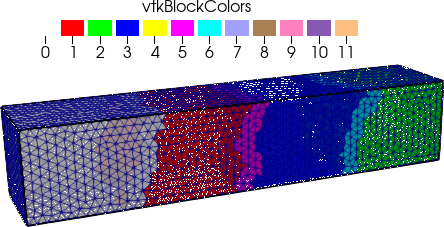
\includegraphics[align=b,width=1\textwidth]{./Images/3d-bar-clamped-ends.png}
    \end{minipage}\hspace{.1\textwidth}
    \begin{minipage}[t][2cm][t]{0.4\textwidth}
    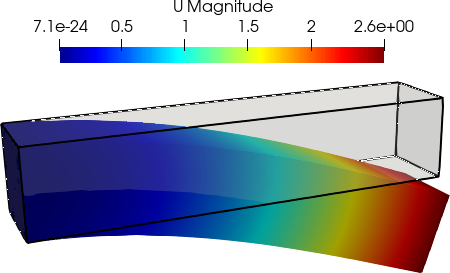
\includegraphics[align=b,width=1\textwidth]{./Images/3d-bar-clamped-pulled-partioned.png}
    \end{minipage}
    \caption{3D bar results. Partitioned mesh (left) and 0.5X warped displacement field (right).}
    \label{fig:3Dpart}
\end{figure}

In \cref{fig:3Dpart} there are four subdomais in the partitioned mesh
since four cores were used.

}


\subsection{PSD simulation of 3D  mechanical piece (Dirichlet-Neumann case) with complex mesh\label{sec:3d-bar-clamped3-sub}}

{
	\renewcommand{\subsection}{\subsubsection}
	\newcommand{\psd}[1]{{\small\sffamily{\color{blue!60}#1}}}

So far in the previous cases we only concentrated on bar simulations,
which were more or less trivial cases. Moreover, the bar meshes are
provided with the PSD solver. In this section we now turn towards 3D
simulation of a mechanical piece, the geometry of which is shown
in\textasciitilde{}\cref{fig:mechanicalpiecegeo}. The left (small) hole
is fixed: \(u_1=u_2=u_3=0\), while as traction force \(t_x=10^9\) is
applied on the large hole.

You can grab a copy of CAD geometry for the mechanical piece (the Gmsh
\psd .geo\}) your local Gmsh installation folder
\psd gmsh/share/doc/gmsh/demos/simple\_geo/\{piece\}.geo\}. The listing
of the file is also given in @. To generate the mesh \psd piece.msh\}
simply do

\begin{lstlisting}[style=BashInputStyle]
gmsh -3 piece.geo
\end{lstlisting}

Place the generated mesh \psd piece.msh\} in
\psd /PSD/Meshes/3D/piece.msh\}. Now the PSD simulation can be
performed.

\begin{figure}[h]
    \centering
    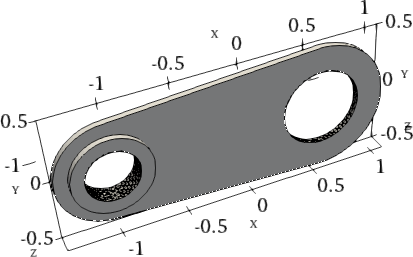
\includegraphics[align=b,width=0.5\textwidth]{./Images/3d-mechanical.png}
    \caption{3D mechanical piece.}
    \label{fig:mechanicalpiecegeo}
\end{figure}

\textbf{Step 1: Preprocessing}

For ``PSD setup'' go to any folder, launch the terminal there and run
the following command.

\begin{lstlisting}[style=BashInputStyle]
PSD_PreProcess  -problem linear-elasticity -dimension 3 -dirichletconditions 1 -tractionconditions 1 -postprocess u
\end{lstlisting}

Here, by using these parameters we have generated one Dirichlet
condition and one traction condition, respectively to be applied to the
small and the large holes in the mesh. Further, by using \psd -dimension
3\} we have let PSD know that the problem is 3D .In the
\psd /PSD/Meshes/3D/piece.msh\} generated, the label 4
(resp.\textasciitilde{}3) corresponds to the Dirichlet
(resp.\textasciitilde{}traction) border. To provide Dirichlet conditions
on label number 4 (\(u_x=0,u_y=0,u_z=0\)) in
\psd ControlParameters.edp\} use set \psd Dbc0On 4\}, \psd Dbc0Ux 0.\},
\psd Dbc0Uy 0.\}, and \psd Dbc0Uz 0.\}. To add the values and label
numbers of the traction borders edit the \psd ControlParameters.edp\},
set \psd Tbc0On 3\} and \psd Tbc0Ty -1.e9\}. For this end
\(\mathbf t=[t_x,t_y,t_z]=[0.,10^9,0.]\). Finally we use steel
properties for the material, so in \psd ControlParameters.edp\} the
parameters \psd real E = 200.e9;\} and \psd real nu = 0.3;\} should be
used. These represent \(E\) and \(\nu\), respectively. With all the
properties and boundary conditions set we now use \psd string ThName =
``../Meshes/3D/piece'';\} in the \psd ControlParameters.edp\} file, this
notifies PSD about the name of the mesh used for this simulation.

\textbf{Step 2: Solving}

Let us now use 2 cores to solve this problem. To do so enter the
following command:

\begin{lstlisting}[style=BashInputStyle]
PSD_Solve -np 2 Main.edp
\end{lstlisting}

\textbf{Step 3: Postprocessing}

Launch ParaView and have a look at the \psd .pvd\} file in the
\psd PSD/Solver/VTUs\_DATE\_TIME\} folder.

\begin{figure}[htbp]
    \centering
    \begin{minipage}[t][2cm][t]{0.36\textwidth}
    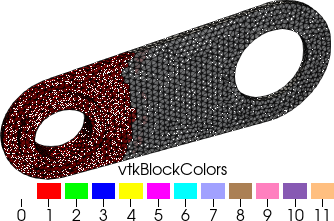
\includegraphics[align=b,width=1\textwidth]{./Images/3d-mechanical-part.png}
    \end{minipage}\hspace{.1\textwidth}
    \begin{minipage}[t][2cm][t]{0.4\textwidth}
    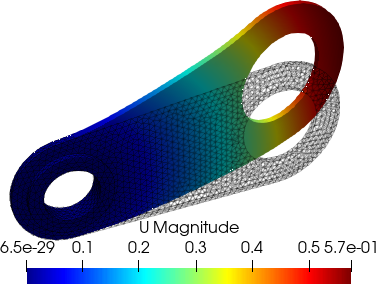
\includegraphics[align=b,width=1\textwidth]{./Images/3d-mechanical-result.png}
    \end{minipage}
    \caption{Mechanical piece test results. Partitioned mesh (left) and  warped displacement field (right).}
    \label{fig:mechapieceresult}
\end{figure}

\textbf{Redoing the test with different conditions}

\begin{figure}[htbp]
    \centering
    \begin{minipage}{0.42\textwidth}
    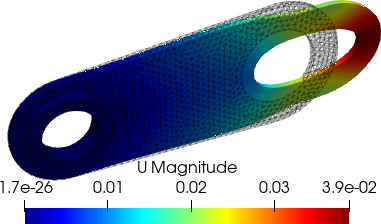
\includegraphics[align=b,width=1\textwidth]{./Images/3d-mechanical-result-x.png}
    \end{minipage}
    \caption{Mechanical piece test results: \psd{ real  tx0=1.e9, ty0=0, tz0=0.,;}}
\end{figure}

\begin{figure}[htbp]
    \centering        
    \begin{minipage}{0.4\textwidth}
    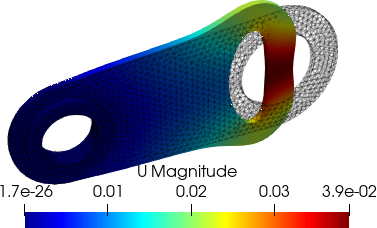
\includegraphics[align=b,width=1\textwidth]{./Images/3d-mechanical-result--x.png}
    \end{minipage}
    \caption{Mechanical piece test results:\psd{ real  tx0=1.e9, ty0=0, tz0=0.,;}}
    \label{fig:mechapieceresult2}
\end{figure}

}


\subsection{PSD linear elasticity tutorial using Mfront-PSD interface\label{sec:2d-mfront}}

{
\renewcommand{\subsection}{\subsubsection}
\newcommand{\psd}[1]{{\small\sffamily{\color{blue!60}#1}}}

This tutorial details one to use PSD-MFront interface for linear
elasticity problem. The same problem from tutorial 1 is repeated,
however now MFront is used for building certain finite element
essentials. It is advised to follow this tutorial after tutorial 1. Note
that, linear elasticity merely provides means of getting started with
Mfornt, the real potential lies in using nonlinear materials and laws
which Mfront provides. So this tutorial should be considered as baptism
to the world of PSD-MFront which we believe has a lot of potential to
solve some non trivial problems.

We reintroduce the problem from tutorial 1, an example of a 2D bar which
bends under its own load -- typical case of linear elasticity. A bar 5 m
in length and 1 m in width, and is supposed to be made up of a material
with density \(\rho=8\times 10^3\), Youngs modulus \(E=200\times 10^9\),
and Poissons ratio \(\nu=0.3\).

\begin{figure}[h!]
\centering
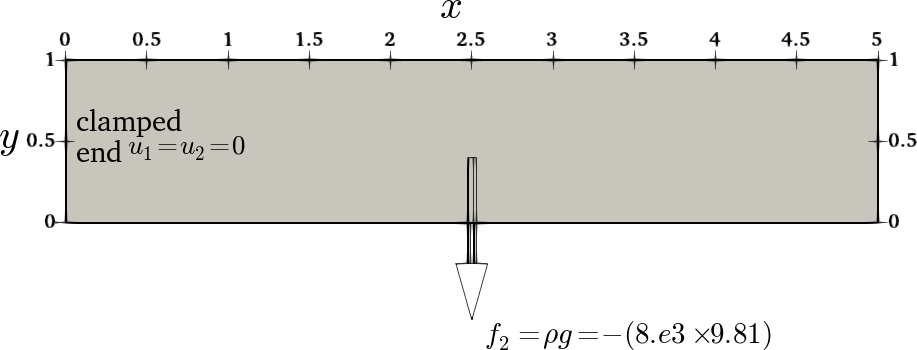
\includegraphics[width=0.5\textwidth]{./Images/le-2d-bar.png}
\caption{The 2D clamped bar problem. \label{2dbar-le-full-mfront}}
\end{figure}

\subsection{Step 1: Preprocessing}

First step in a PSD simulation is PSD preprocessing, at this step you
tell PSD what kind of physics, boundary conditions, approximations,
mesh, etc are you expecting to solve. More importantly for this tutorial
we will signify to PSD that MFront has to be used.

In the terminal \psd{cd} to the folder
\psd{/home/PSD-tutorials/linear-elasticity}. Launch
\psd{PSD\_PreProcess} from the terminal, to do so run the following
command.

\begin{lstlisting}[style=BashInputStyle]
PSD_PreProcess -problem linear_elasticity -dimension 2 -bodyforceconditions 1 \
-dirichletconditions 1 -postprocess u -useMfront
\end{lstlisting}

After the \psd{PSD\_PreProcess} runs successfully you should see many
\psd{.edp} files in your current folder.

\textbf{What do the arguments mean ?}

\begin{itemize}
\item \psd{-problem linear\_elasticity} means that we are solving linear elasticity problem;
\item \psd{-dimension 2} means it is a 2D simulation;
\item \psd{-bodyforceconditions 1} with applied body force acting on the domain;
\item \psd{-dirichletconditions 1} says we have one Dirichlet border;
\item \psd{-postprocess u} means we would like to have ParaView post processing files.
\item \psd{-useMfront} activates MFront interface for PSD.
\end{itemize}

At this stage the input properties \(E,\nu\) can be mentioned in
\psd{ControlParameters.edp}, use \psd{E = 200.e9}, and \psd{nu = 0.3}.
In contrast to tutorial 1, notice that these values of \psd{E} and
\psd{nu} are fed to a vector \psd{PropertyValues = [E, nu];} verbosed by
\psd{PropertyNames   = "YoungModulus PoissonRatio";}. We also signify
that we will be solving linear elasticity via
\psd{MforntMaterialBehaviour   = "Elasticity";} and also
\psd{MaterialHypothesis = "GENERALISEDPLANESTRAIN";} which signifies the
hypothesis to be used for the Linear elasticity
\footnote{The \psd{MaterialHypothesis} accepts \psd{"GENERALISEDPLANESTRAIN"},  \psd{"PLANESTRAIN"}, \psd{"PLANESTRESS"},  and  \psd{"TRIDIMENSIONAL"} as arguments.}.
\psd{PropertyValues}, \psd{PropertyNames}, and \psd{MaterialHypothesis}
will eventually be provided to MFront in \psd{FemParameters.edp} file
via \psd{mfrontElasticityHandler(...)} function
\footnote{User is encouraged to have a look at \psd{FemParameters.edp} file.}.
The volumetric body force condition is mentioned in the same file via
variable \psd{Fbc0Fy -78480.0}, i.e (\(\rho*g=8.e3*(-9.81)=-78480.0\)).
One can also provide the mesh to be used in \psd{ControlParameters.edp},
via \psd{ThName = "../Meshes/2D/bar.msh"}
(\textit{note that mesh can also be provided in the next step}) .In
addition variable \psd{Fbc0On 1} has to be provided in order to indicate
the volume (region) for which the body force is acting, here \psd{1} is
the integer volume tag of the mesh. Dirichlet boundary conditions are
also provided in \psd{ControlParameters.edp}. To provide the clamped
boundary condition the variables \psd{Dbc0On 2}, \psd{Dbc0Ux 0.}, and
\psd{Dbc0Uy 0.} are used, which means for Dirichlet border \psd{2}
(\psd{Dbc0On 2}) where \psd{2} is the clamped border label of the mesh
Dirichlet constrain is applied and \psd{Dbc0Ux 0.}, \psd{Dbc0Uy 0} i.e.,
the clamped end condition (\(u_x=u_y=0\)).

\subsection{Step 2: Solving}

As PSD is a parallel solver, let us use 4 cores to solve the 2D bar
case. To do so enter the following command:

\begin{lstlisting}[style=BashInputStyle]
PSD_Solve -np 4 Main.edp -mesh ./../Meshes/2D/bar.msh -v 0
\end{lstlisting}

Here \psd{-np 4} denote the argument used to enter the number of
parallel processes (MPI processes) used while solving.
\psd{-mesh ./../Meshes/2D/bar.msh} is used to provide the mesh file to
the solver. \psd{-v 0} denotes the verbosity level on screen.
\psd{PSD\_Solve} is a wrapper around \psd{FreeFem++-mpi}. Note that if
your problem is large use more cores. PSD has been tested upto 13,000
parallel processes and problem sizes with billions of unknowns, surely
you will now need that many for the 2D bar problem.

\subsection{Step 3: Postprocessing}

PSD allows postprocessing of results in ParaView. After the step 2
mentioned above finishes. Launch ParaView and have a look at the
\psd{.pvd} file in the \psd{VTUs...} folder. Using ParaView for
postprocessing the results that are provided in the \psd{VTUs...}
folder, results such as those shown in \cref{bar-le-full-mfront-pv} can
be extracted.

\begin{figure}[h!]
\centering
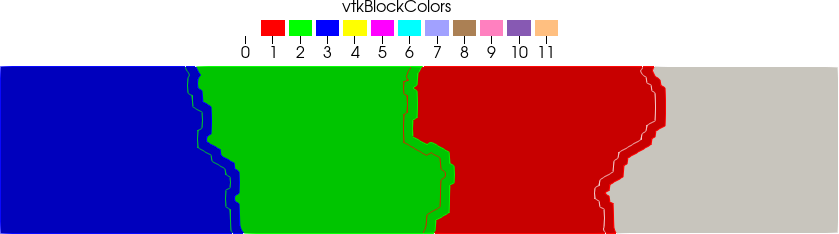
\includegraphics[align=t,width=0.4\textwidth]{./Images/le-2d-bar-partioned.png}\hfill
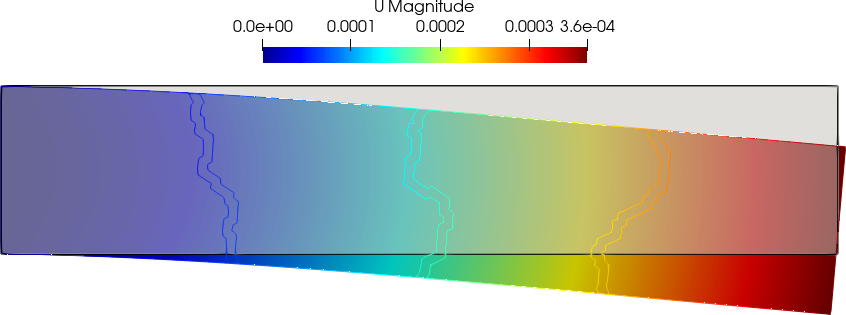
\includegraphics[align=t,width=0.4\textwidth]{./Images/le-2d-bar-results.png}
\caption{The 2D clamped bar problem: partitioned mesh and displacement field visualization in ParaView. \label{bar-le-full-mfront-pv}}
\end{figure}

You are all done with your 2D linear-elasticty simulation with Mfront
interface.

\subsection{How and what is being done in PSD-MFront interface? }

To explain how PSD-MFront interface works we will compare how a PSD
solver acts when using MFront or without. In other words what is
different when \psd{-useMfront} is used at preprocessing. Note that
ultimately the problem results (displacement fields, stresses, strains)
will be the same.

To put it briefly, what MFront does for linear elasticity problem here
is build the Material tensor (stiffness matrix) at each quadrature
point. So, there are two points

\begin{itemize}
\item We need to communicate to Mfront the nature of the problem and the material involved.
\item We need to provide Mfornt the stiffness matrix at each quadrature point so that it can fill it up.
\end{itemize}

The two raised points are handled using
\psd{mfrontElasticityHandler(...)} in \psd{FemParameters.edp} file.

Firstly, the arguments \psd{E = 200.e9}, \psd{nu = 0.3},
\psd{MforntMaterialBehaviour   = "Elasticity";},
\psd{PropertyValues = [E, nu];},
\psd{PropertyNames   = "YoungModulus PoissonRatio";},
\psd{PropertyValues = [E, nu];} and
\psd{MaterialHypothesis = "GENERALISEDPLANESTRAIN";} form
\psd{ControlParameters.edp} takes care of the first point (the nature of
the problem and the material involved). The latter three arguments well
define that we have a 2D problem, with given values of properties
(\(E, \nu\)). The snippet from \psd{ControlParameters.edp} (produced
after using \psd{-useMfront} argument for \psd{PSD\_PreProcess}) file
shows these variables which define the nature of the problem and
characteristics of material involved

\begin{lstlisting}[style=CppStyle]
//============================================================================
//                   ------- Material parameters -------
// -------------------------------------------------------------------
//  E, nu : Modulus of Elasticity and Poisson ratio of the material
//  PropertyNames : String of material property names (space seperated)
//                  that are provided to Mfront.
//  PropertyValues : Values of material properties provided to Mfront
//
// -------------------------------------------------------------------
//  NOTE:     Please note that PropertyNames should be the same as
//            as in the Elasticity.mfront file
// -------------------------------------------------------------------
//============================================================================

  macro E()  200.e9  //
  macro nu() 0.3     //

  string    MaterialBehaviour  = "Elasticity";
  string    MaterialHypothesis = "GENERALISEDPLANESTRAIN";
  string    PropertyNames      = "YoungModulus PoissonRatio";
  real[int] PropertyValues     = [ E, nu ];
\end{lstlisting}

Secondly, the to get the stiffness matrix from Mfornt we use a
quadrature finite element space with vector finite elements built on it
(6 components) that represent the 6 components of symmetric material
tensor (\(\mathbb R^{3 \times 3}\)). The snippet from
\psd{MeshAndFeSpace.edp} file shows the 6 component Quadrature finite
element space for building material tensor.

\begin{lstlisting}[style=CppStyle]
//==============================================================================
// ------- The finite element space  -------
// ----------------------------------------------------------------------------
//  Qh       : Quadratur finite element space  for material tensor
//             FEQF2 implies 3 dof for a triangular cell in the mesh
//             A vectorial FEM space is built with 6 components
//==============================================================================

 fespace Qh  ( Th ,[ FEQF2, FEQF2, FEQF2,
                           FEQF2, FEQF2,
                                  FEQF2] );
\end{lstlisting}

Finally in file \psd{FemParameters.edp} the
\psd{mfrontElasticityHandler()} is called to build the material tensor
\psd{Mt} provided with the previously built material properties and
nature of problem. Please see the snippet below

\begin{lstlisting}[style=CppStyle]
//============================================================================
// ------- Material Tensor using Quadrature FE space -------
// -------------------------------------------------------------------
// Mt[int]  : is an array of finite element variable belonging to quadratu
//            re space Qh. This array is used  to define components of the
//            material tensor. 3X3 in 2D and 6X6 in 3D
//            In 2D the material tensor looks like
//
//         [ 2*mu+lambda ,  lambda      , 0 ]    [ Mt11 , Mt12 , Mt13 ]
//   Mt =  [ lambda      ,  2*mu+lambda , 0 ] =  [ Mt12 , Mt22 , Mt23 ]
//         [   0         ,     0        , mu]    [ Mt13 , Mt23 , Mt33 ]
//
// mfrontElasticityHandler : is a function in mfront interface that helps
//                           building the material tensor  Mt  given with
//                           material prpts.  from  ControlParameters.edp
//============================================================================

  Qh [ Mt11 ,  Mt12 , Mt13 ,
              Mt22 , Mt23 ,
                     Mt33 ];


  mfrontElasticityHandler( MforntMaterialBehaviour                             ,
                           mfrontBehaviourHypothesis = MaterialHypothesis      ,
                           mfrontPropertyNames       = PropertyNames           ,
                           mfrontPropertyValues      = PropertyValues          ,
                           mfrontMaterialTensor      = Mt11[]
                         );
\end{lstlisting}

Note that in the snippet above you might be seeing \psd{Mt11[]} being
provided as \psd{mfrontMaterialTensor}, in fact the \psd{Mt11[]} calls
the full matrial tensor not just the first component, so user should not
get confused
\footnote{This is more technical note, \psd{Mt11[]} is the cast of \psd{Mt} vector to a single array for memory optimization. One can also simply use \psd{Mt12[]}, \psd{Mt13[]}, \psd{Mt22[]}, ... all these are acceptable and are simply aliases to material tensor.}.

The material tensor \psd{Mt} built is used in the finite element
variational formulation to build the bilinear
\(a(\mathbf{u},\mathbf{v})\) which is used to assemble the finite
element matrix \(\mathbf{A}\) for the linear system
\(\mathbf{Ax} = \mathbf{b}\)

\[
a(\mathbf{u},\mathbf{v}) = \int_{\Omega}(
                 \varepsilon \left(\mathbf{u}):\mathbf{Mt}:\varepsilon(\mathbf{v}\right)
               )
\]

Here, \(\varepsilon(\mathbf{u}):\mathbf{Mt}\) is nothing but the stress
\(\sigma(\mathbf{u})\) operator. User is encourage to have a look at the
\psd{VariationalFormulation.edp} file that contains the variational
formulation (weak form) of the problem described.

}


\subsection{Additional exercises on linear elasticity}
{
	\renewcommand{\subsection}{\subsubsection}
	\newcommand{\psd}[1]{{\small\sffamily{\color{blue!60}#1}}}

\subsection{Advance exercise  1}

There is a solver run level flag for mesh refinement
\footnote{Mesh refinement is performed after partitioning.}. This flag
is called \psd{-split [int]} which splits the triangles (resp.
tetrahedrons) of your mesh into four smaller triangles (resp.
tetrahedrons). As such \psd{-split 2} will produce a mesh with 4 times
the elements of the input mesh. Similarly, \psd{-split n} where \(n\) is
a positive integer produces \(2^n\) times more elements than the input
mesh. You are encouraged to use this \psd{-split} flag to produce
refined meshes and check, mesh convergence of a problem, computational
time, etc. Use of parallel computing is recommended. You could try it
out with \psd{PSD\_Solve} or \psd{PSD\_Solve\_Seq}, for example:

\begin{lstlisting}[style=BashInputStyle]
PSD_Solve -np 4 Main.edp -mesh ./../Meshes/2D/bar.msh -v 0 -split 2
\end{lstlisting}

for splitting each triangle of the mesh \psd{bar.msh} into 4.

\subsection{Advance exercise  2}

There is a preprocess level flag \psd{-debug}, which as the name
suggests should be used for debug proposes by developers. However, this
flag will activate OpenGL live visualization of the problems
displacement field. You are encouraged to try it out

\begin{lstlisting}[style=BashInputStyle]
PSD_PreProcess -problem linear_elasticity -dimension 2 -bodyforceconditions 1 \
-dirichletconditions 1 -postprocess u -timelog -debug
\end{lstlisting}

Then to run the problem we need additional \psd{-wg} flag

\begin{lstlisting}[style=BashInputStyle]
PSD_Solve -np 4 Main.edp -mesh ./../Meshes/2D/bar.msh -v 0 -wg
\end{lstlisting}

\subsection{Advance Exercise  3}

One interesting way of solving a linear Elasticity problem is to solve
it via a pseudo nonlinear model. There is a preprocess level flag
\psd{-model pseudo\_nonlinear}, which introduces pseudo nonlinearity
into the finite element variational formulation of linear elasticity.
You are encouraged to use this flag and see how the solver performs.
Indeed, now you should see some nonlinear iterations (1 or 2) are taken
for convergence.

\begin{lstlisting}[style=BashInputStyle]
PSD_PreProcess -problem linear_elasticity -dimension 2 -bodyforceconditions 1 \
-dirichletconditions 1 -postprocess u -timelog -model pseudo_nonlinear
\end{lstlisting}

Then to run the problem

\begin{lstlisting}[style=BashInputStyle]
PSD_Solve -np 4 Main.edp -mesh ./../Meshes/2D/bar.msh -v 0
\end{lstlisting}

To understand what the flag does, try to find out the difference between
the files created by \psd{PSD\_PreProcess} when used with and without
\psd{-model pseudo\_nonlinear} flag. Especially, compare
\psd{LinearFormBuilderAndSolver.edp} and
\psd{VariationalFormulations.edp} files produced by
\psd{PSD\_PreProcess} step. You will see Newton--Raphsons iterations are
performed for solving the linear problem. However, the nonlinear
iterations loop converges very rapidly (in 1 iteration) due to linear
nature of the problem. \textbf{Note:} This flag is exclusive for
parallel solver.

\subsection{Advance exercise 4}

There is a preprocess level flag \psd{-withmaterialtensor}, which
introduces the full material tensor into the finite element variational
formulation. You are encouraged to use this flag and see how the solver
performs.

\begin{lstlisting}[style=BashInputStyle]
PSD_PreProcess -problem linear_elasticity -dimension 2 -bodyforceconditions 1 \
-dirichletconditions 1 -postprocess u -timelog -withmaterialtensor
\end{lstlisting}

Then to run the problem

\begin{lstlisting}[style=BashInputStyle]
PSD_Solve -np 4 Main.edp -mesh ./../Meshes/2D/bar.msh -v 0
\end{lstlisting}

To understand what the flag does, try to find out the difference between
the files created by \psd{PSD\_PreProcess} when used with and without
\psd{-withmaterialtensor} flag. Especially, compare
\psd{FemParameters.edp}, \psd{MeshAndFeSpace} and
\psd{VariationalFormulations.edp} files produced by
\psd{PSD\_PreProcess} step.

}

\pagebreak

\section{Damage mechanics}
\subsection{Hybrid phase-field for damage}
On a meshed domain $\Omega^h\in\Omega\subset\mathbb{R}^n$, for damage mechanics the mixed finite element variational formulation in the Lagrangian framework for searching the unknown nodal displacements vector $\bu^h=[u_1,u_2,u_3]^\mathsf{T}$ reads,
%
%
\begin{equation}\label{Eq:VarfU}
\begin{aligned}
&\text{search}~\buh\in\mathbb{V}^h \text{~that satisfies}~\forall\, t\in[0,T]:\\
&\int_{\Omega^h}\big[(1-d^h)^2 + \kappa \big]\sig(\buh) : \eps(\bvh) \,\dv= \int_{\partial\Omega^h_\text{N}} \overline{\bt}\cdot\bvh \,\ds \quad\forall\,\bv^h\in\mathbb{V}^h,
\end{aligned}
\end{equation}
where $\kappa\ll1$ is a model parameter to prevent numerical singularity when $d \to 1$.
 %
 %
In this formulation, the notation ``$:$'' is used for the double contraction between tensors (i.e., component-wise tensor product) and $ \mathbb{V}^h $ is a  mixed third order vector valued finite element functional space to approximate vector test function~$\bvh$ and vector trial function~$\buh$:
 %
\begin{equation}
\mathbb{V}^h=\left\{ \bu^h\in [ {H}^1(\Omega^h) ]^3~~\forall t\in[0,T]~|~ \forall \bx\in\partial\Omega^h_{\text{D}}~\buh=\overline{\bu}\right\},
\end{equation}
%
with ${H}^1(\Omega^h)$ denoting a square integrable Sobolev functional space.
Similarly, for~the phase-field the standard finite element variational formulation for the unknown damage scalar $\fih$ reads, 
%
%
\begin{equation}
\begin{aligned}\label{Eq:VarfPhi}
&\text{search}~\fih\in{{V}}^h \text{~that satisfies}~\forall\, t\in[0,T]:\\
&\int_{\Omega^h}\left[ \frac{\bgc}{l_0} + 2 \mathcal{H}^{+}(\buh) \right]\fih\ttah\, \dv + \int_{\Omega^h} {\bgc}{l_0}\nabla\fih \cdot \nabla\ttah \, \dv= \int_{\Omega^h} 2\mathcal{H}^{+}(\buh)\ttah \, \dv\quad\forall\,\ttah\in{{V}}^h, 
\end{aligned}
\end{equation}
%
%
where,~${{V}}^h$ denotes the scalar finite element functional space to approximate scalar test function~$\ttah$ and scalar trial function~$\fih$:
\begin{equation}
{{V}}^h=\left\{\fih \in  {H}^1(\Omega^h)~~\forall t\in[0,T]~\middle|~\fih\in[0,1]  \right\}.
\end{equation}


\subsection{Tensile cracking of a pre-cracked plate: A 2D example of PSD parallel solver}


{
	\renewcommand{\subsection}{\subsubsection}
	\newcommand{\psd}[1]{{\small\sffamily{\color{blue!60}#1}}}

A two dimensional test is introduced. The problem of interest is the
typical single notch square plate cracking test under tensile loading. A
unit square with a pre existing crack is clamped at the bottom
\(u_1=u_2=0\) (first boundary condition) and is loaded quasi-statically
\(u_2=u_2 + \Delta u_2\) on its top surface till the crack propagates
through its walls. So there are two Dirichlet conditions one on the top
border and one on the bottom one.

\begin{figure}[h!]
\centering
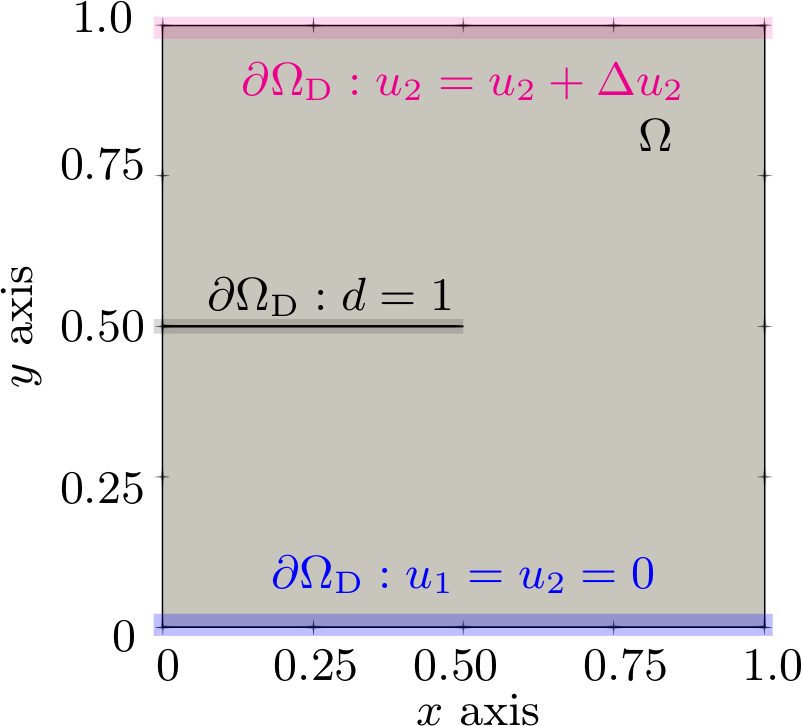
\includegraphics[width=0.3\textwidth]{./Images/square-notch.png}
\caption{Domain of the single notch square cracking problem under tensile loading. \label{bar-sd}}
\end{figure}

To model this test PSD provides hybrid phase-field modelling technique.
We use ParaView post-processing of displacement \(u\) and phase-field
\(d\) to visualise the cracking process. A PSD simulation is a two step
process, with step one being the \psd{ PSD\_PreProcess }:

\begin{lstlisting}[style=BashInputStyle]
PSD_PreProcess -dimension 2 -problem damage -model hybrid_phase_field \
-dirichletconditions 2 -postprocess ud
\end{lstlisting}

A note on flags.

\begin{itemize}
\tightlist
\item
  This is a two-dimensional problem, so we use the flag
  \psd{-dimension 2}.
\item
  This problem indeed falls under the category of damage-mechanics,
  hence the flag \psd{ -problem damage}.
\item
  We wish to solve this problem by invoking the hybrid phase-field
  problem, which is signified by the flag
  \psd{ -model hybrid\_phase\_field}.
\item
  Versed in the description above the problem contains two Dirichlet
  conditions, we signal this via the flag \psd{-dirichletconditions 2}.
\item
  Finally for this problem we use the flag \psd{-postprocess ud} which
  enables post-processing of displacement \(u\) and damage (phase-field)
  \(d\) fields.
\end{itemize}

Once the step above has been performed, we solve the problem using four
MPI processes, with the given mesh file \psd{tensile-crack.msh}. This is
step two of the PSD simulation \psd{ PSD\_Solve}.

\begin{lstlisting}[style=BashInputStyle]
PSD_Solve -np 4 Main.edp -mesh ./../Meshes/2D/tensile-crack.msh -v 0
\end{lstlisting}

\begin{figure}[h!]
\centering

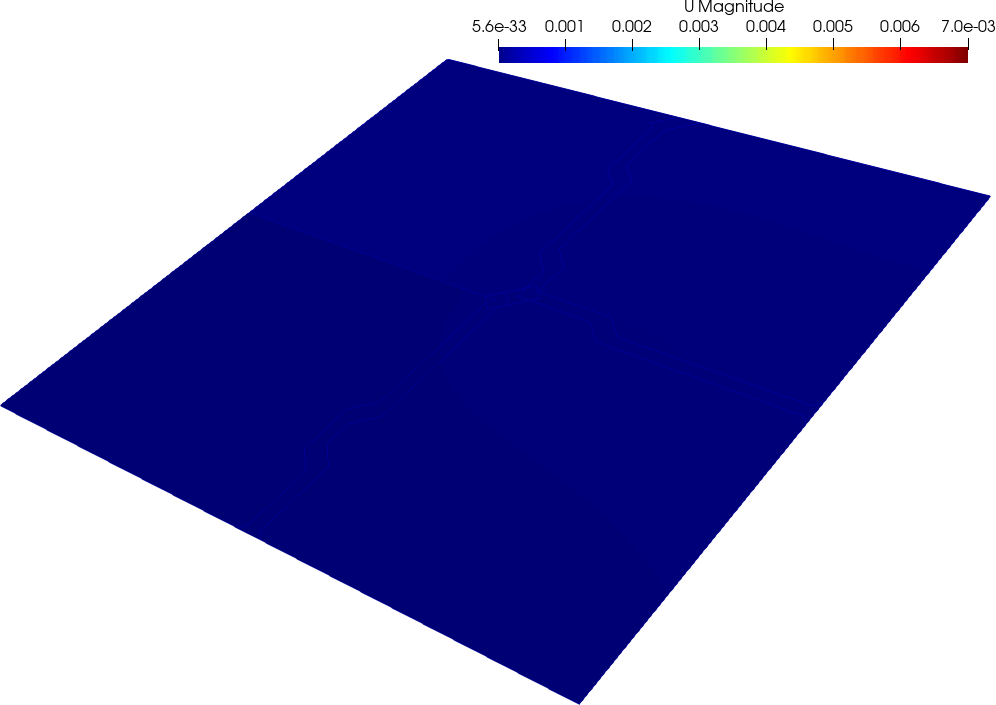
\includegraphics[width=0.24\textwidth]{./Images/u0.png}
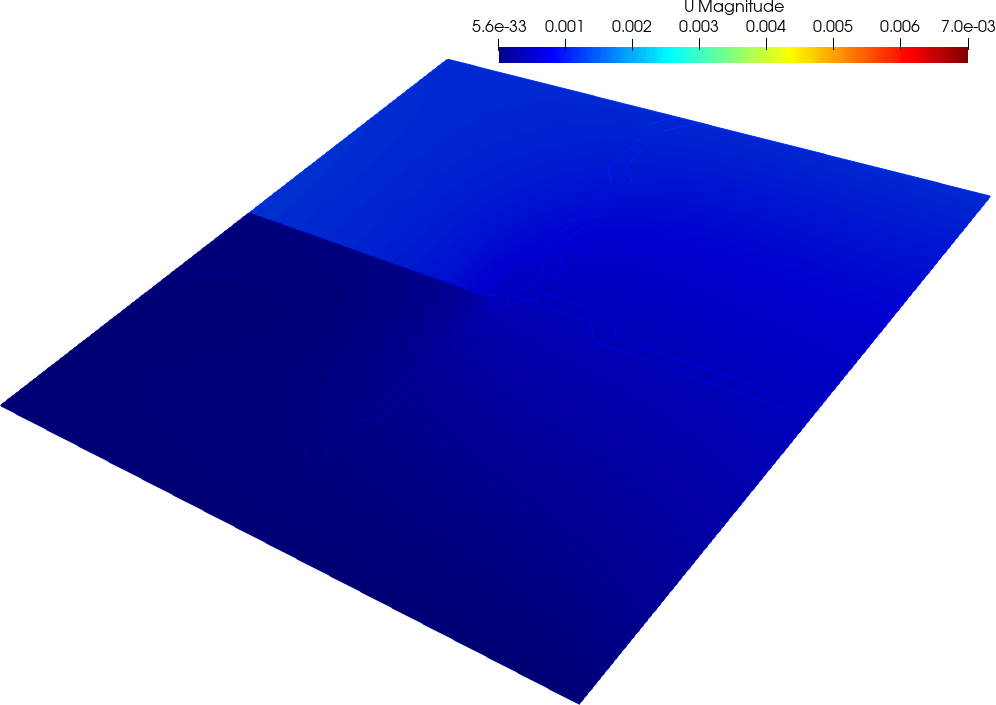
\includegraphics[width=0.24\textwidth]{./Images/u1.png}
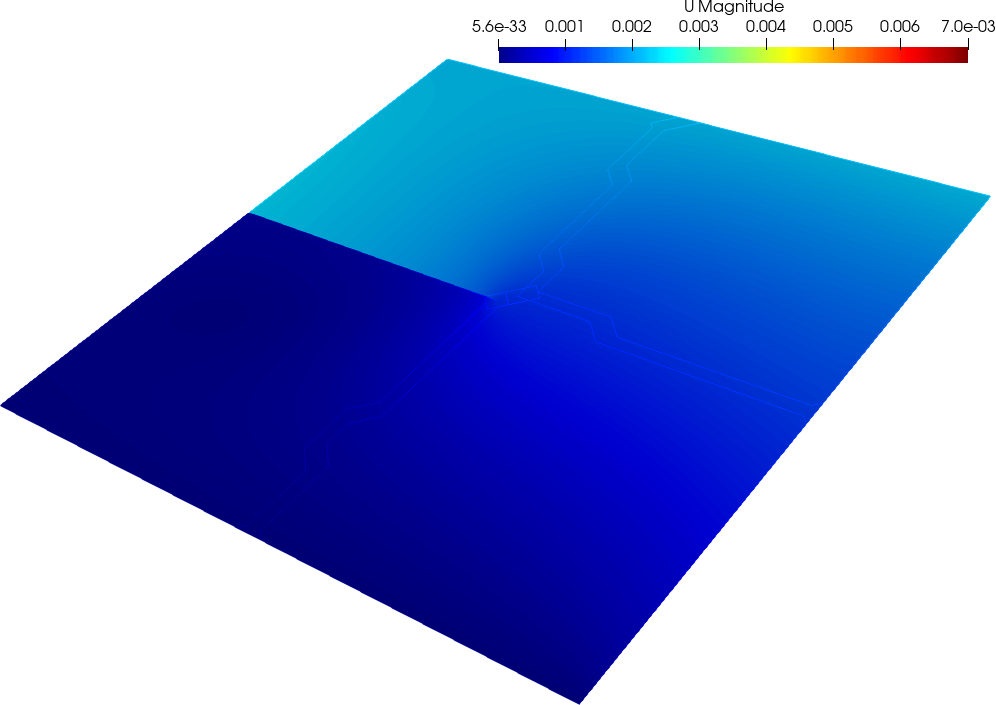
\includegraphics[width=0.24\textwidth]{./Images/u2.png}
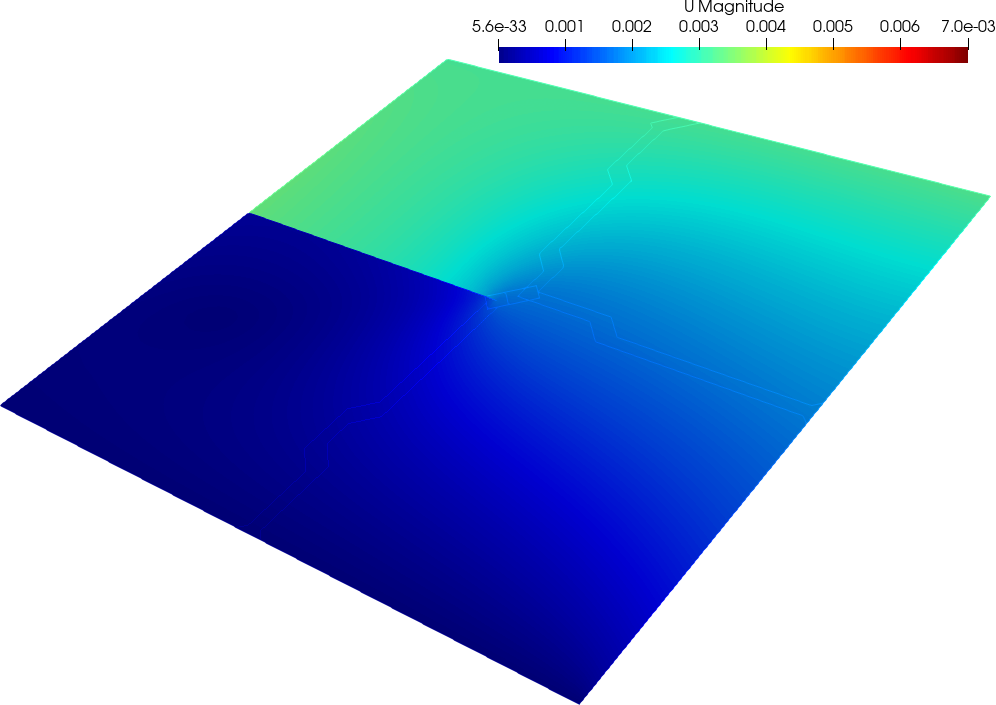
\includegraphics[width=0.24\textwidth]{./Images/u3.png}\\
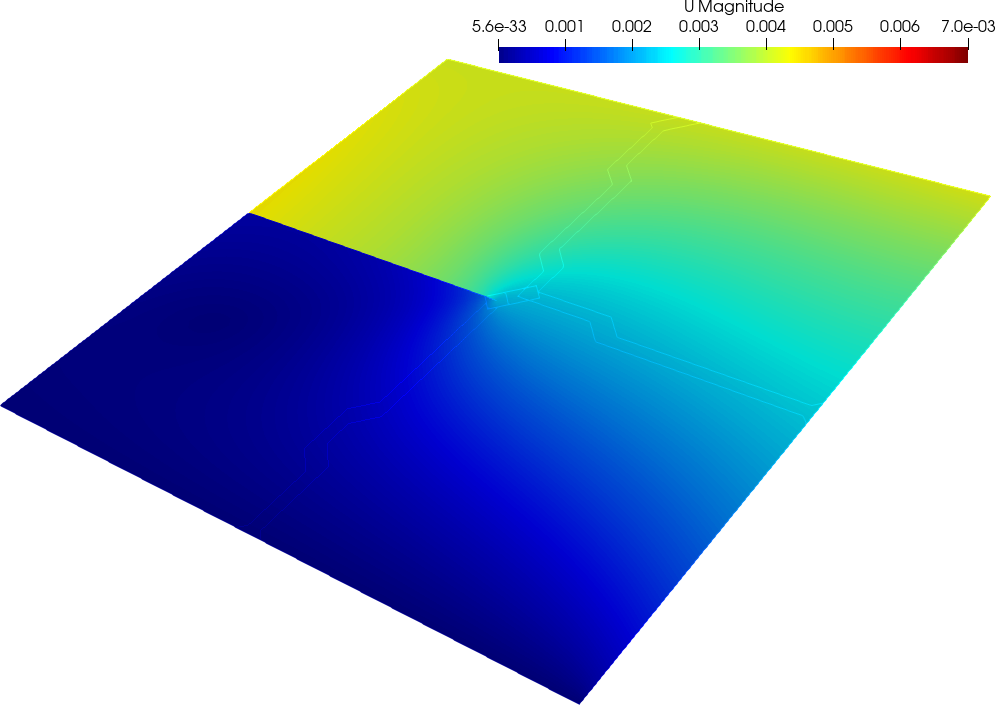
\includegraphics[width=0.24\textwidth]{./Images/u4.png}
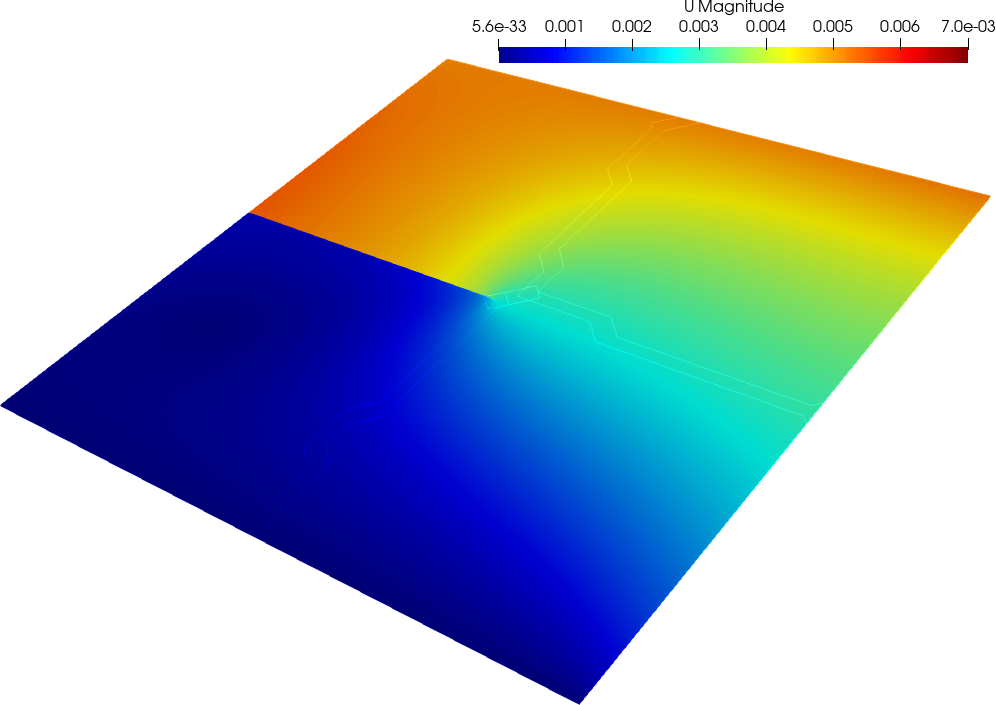
\includegraphics[width=0.24\textwidth]{./Images/u5.png}
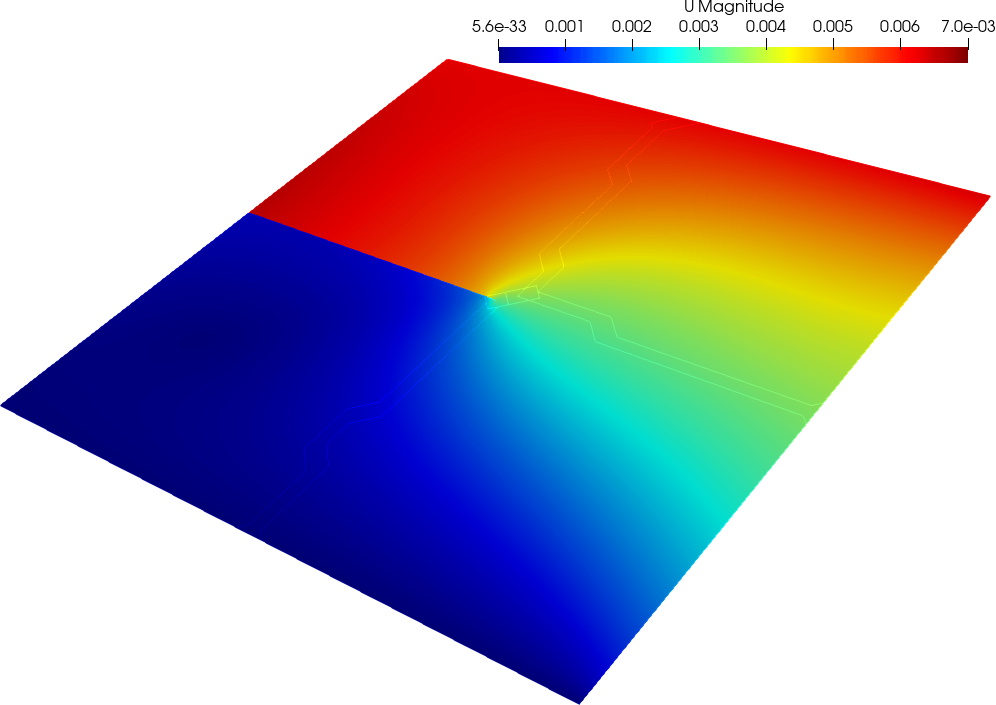
\includegraphics[width=0.24\textwidth]{./Images/u6.png}
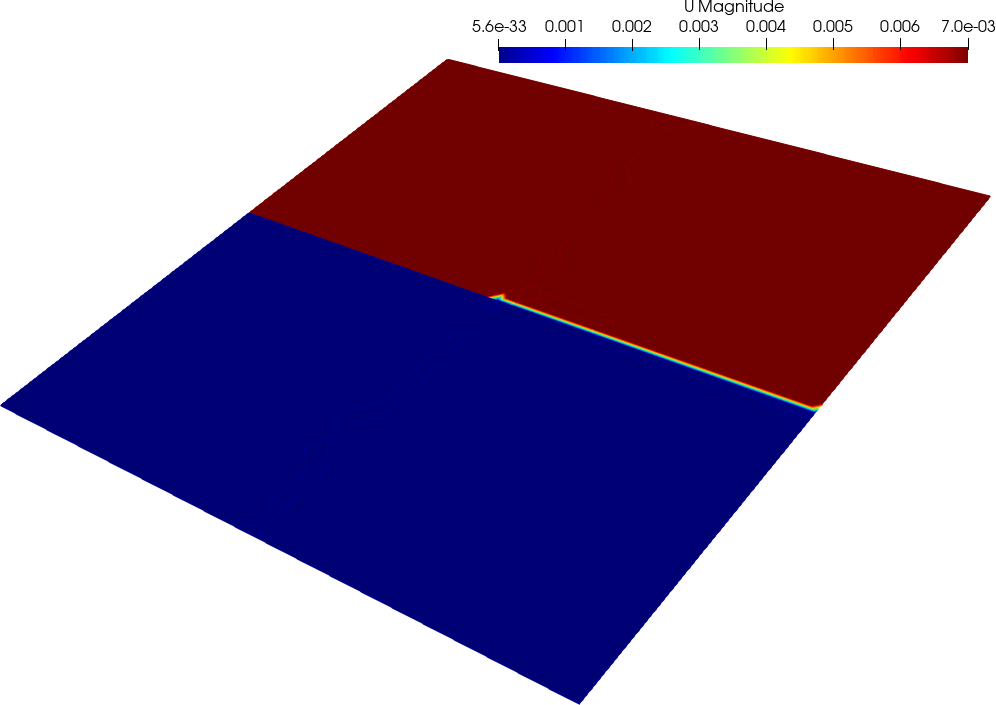
\includegraphics[width=0.24\textwidth]{./Images/u7.png}
\caption{Finite element displacement visualised for the 2D problem with ParaView at different timesteps (quasi-statics). Time progresses from left to right in a row and top to bottom when comparing rows. \label{u-fem}}
\end{figure}

\begin{figure}[h!]
\centering

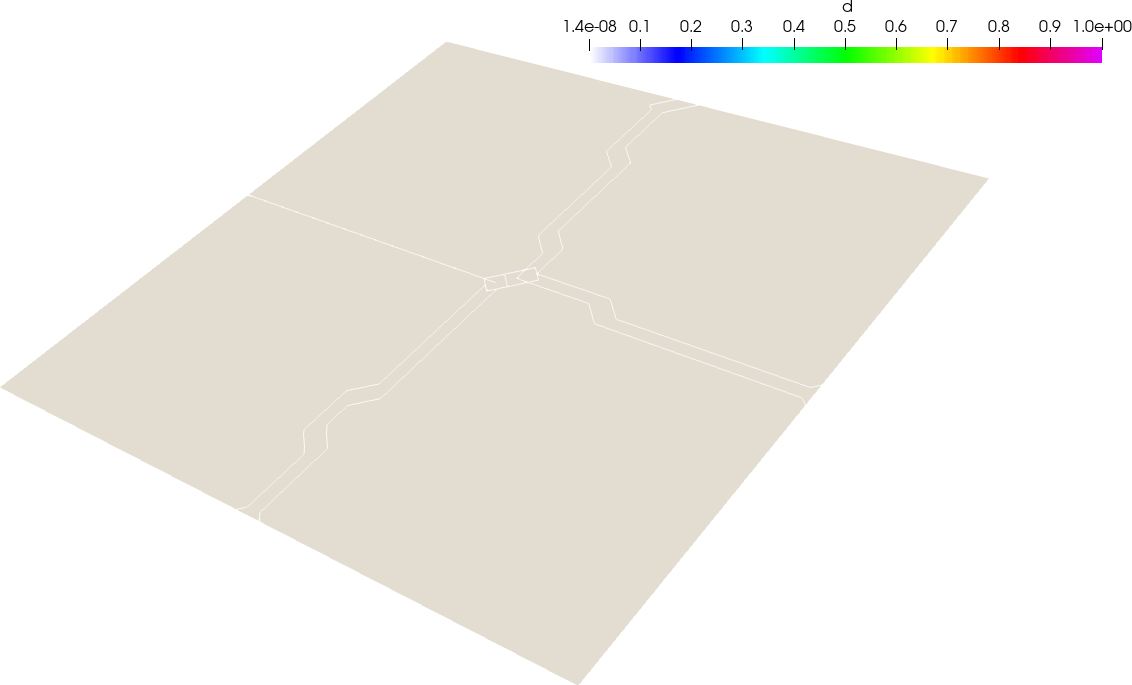
\includegraphics[width=0.24\textwidth]{./Images/d0000.png}
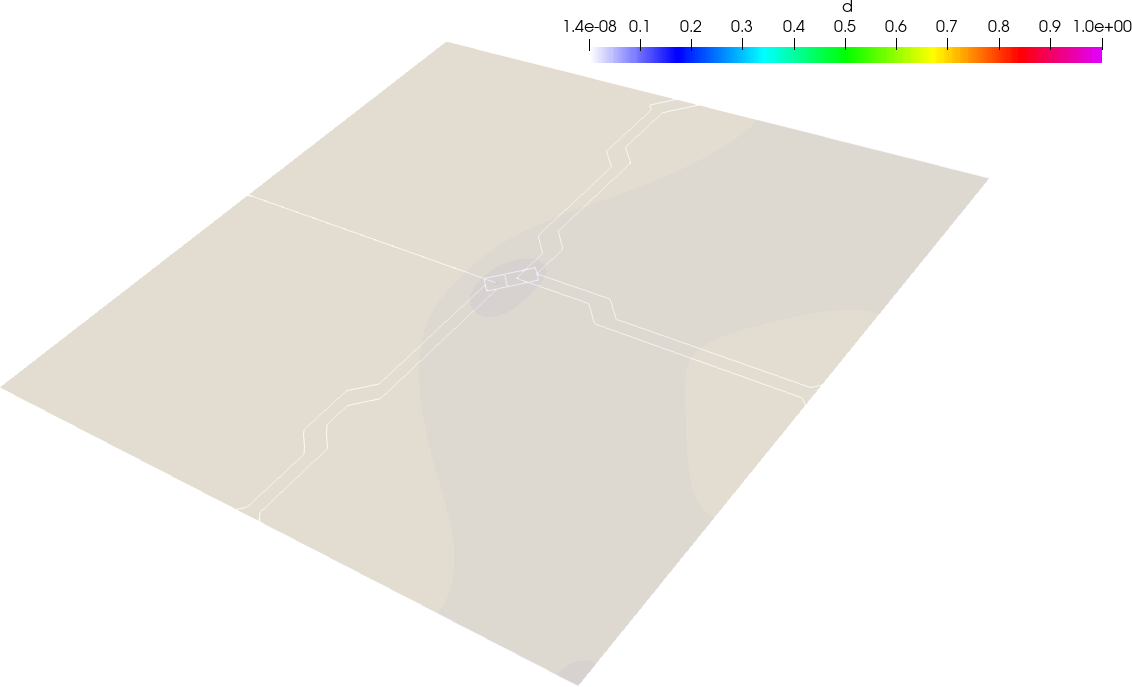
\includegraphics[width=0.24\textwidth]{./Images/d0010.png}
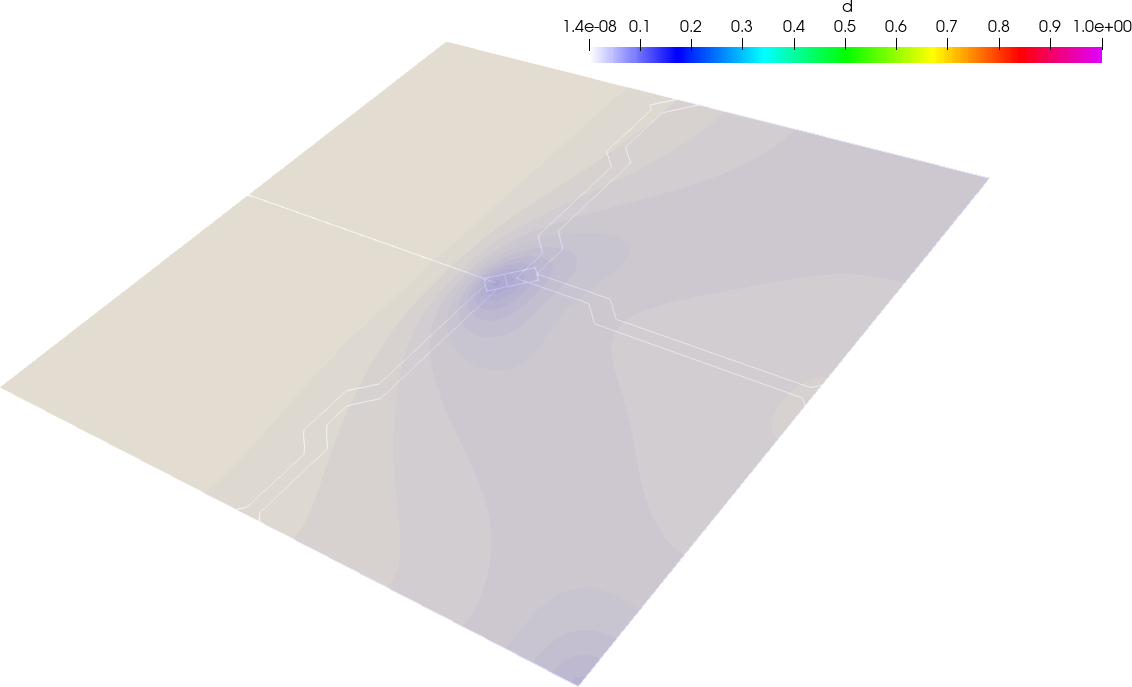
\includegraphics[width=0.24\textwidth]{./Images/d0020.png}
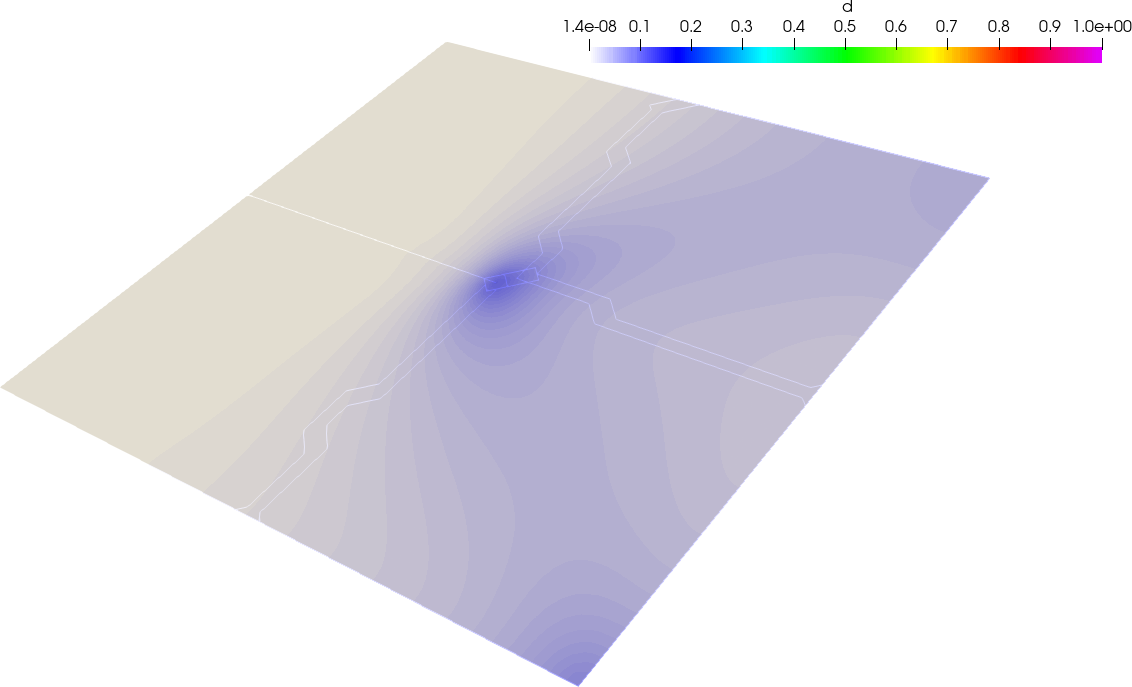
\includegraphics[width=0.24\textwidth]{./Images/d0030.png}\\
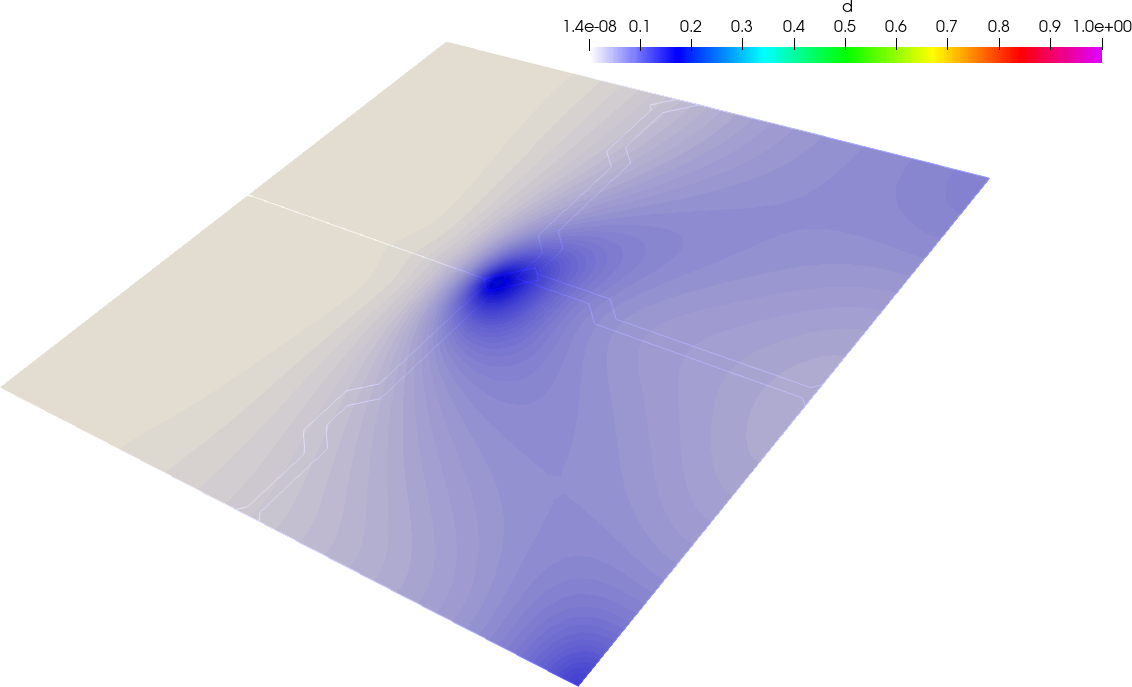
\includegraphics[width=0.24\textwidth]{./Images/d0040.png}
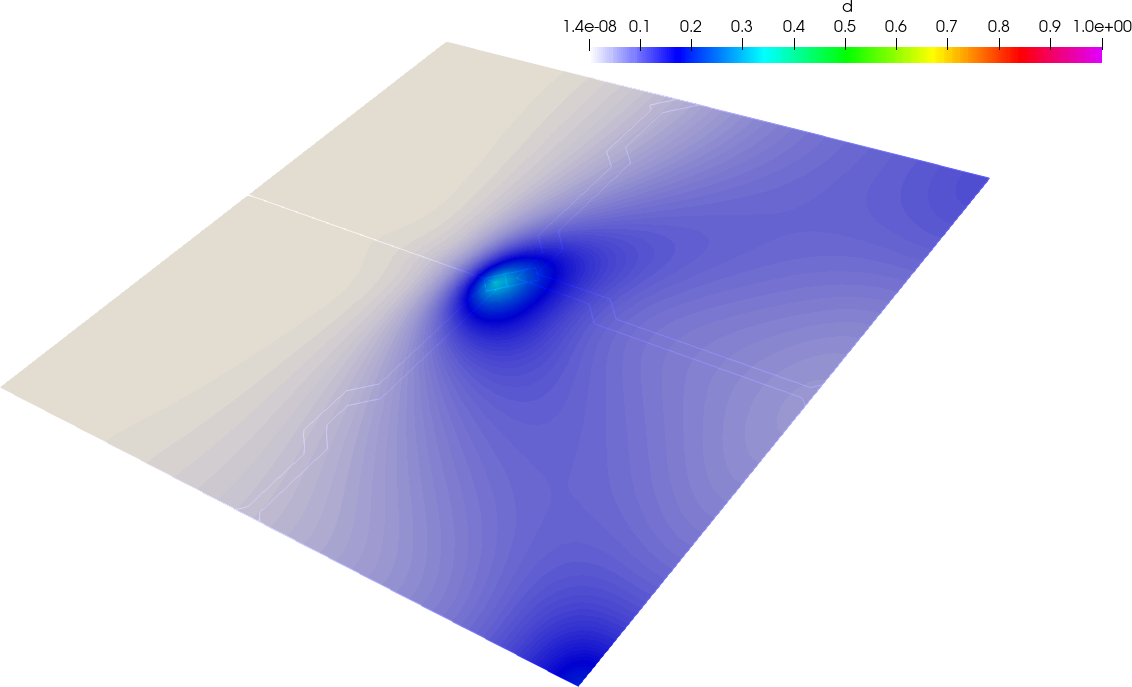
\includegraphics[width=0.24\textwidth]{./Images/d0050.png}
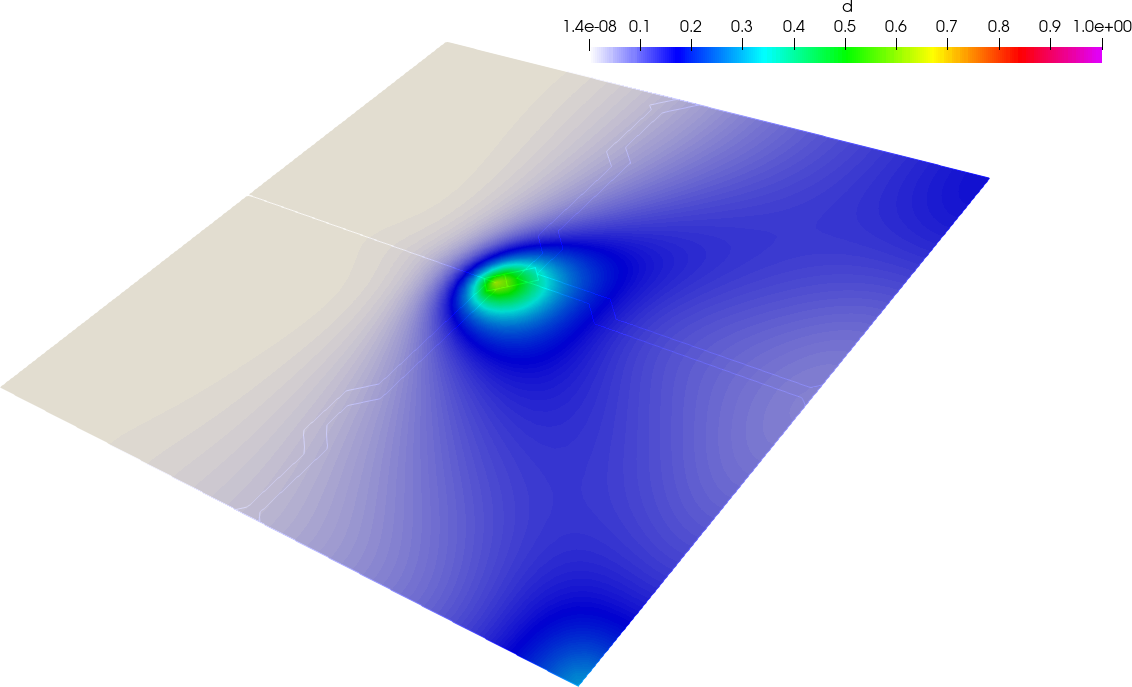
\includegraphics[width=0.24\textwidth]{./Images/d0060.png}
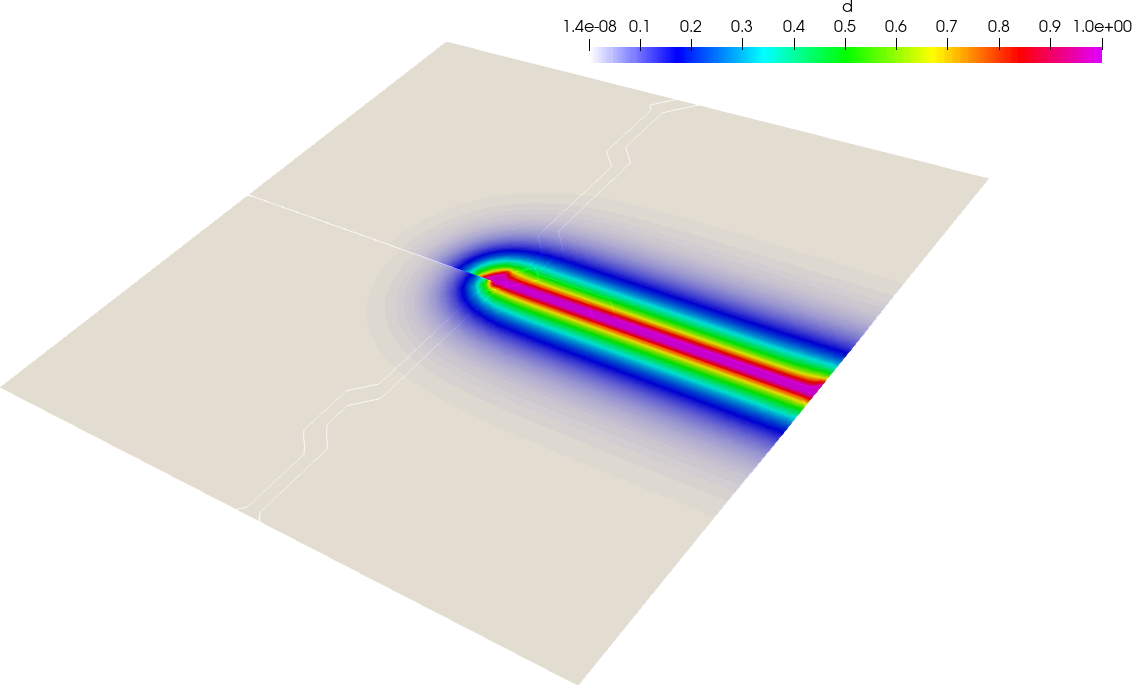
\includegraphics[width=0.24\textwidth]{./Images/d0069.png}
\caption{Finite element damage visualised for the 2D problem with ParaView at different timesteps (quasi-statics). Time progresses from left to right in a row and top to bottom when comparing rows. \label{d-fem}}
\end{figure}

Figures \ref{u-fem} and \ref{d-fem} present the finite element
displacement and damage field, which enable us to visualise the cracking
of the square plate.

\begin{figure}[h!]
\centering

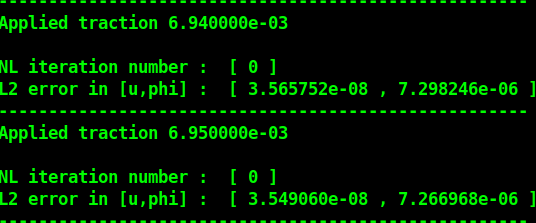
\includegraphics[width=0.6\textwidth]{./Images/terminal1.png}
\caption{Applied traction, non-linear iterations to convergence, and residual being casted onto the terminal shell. \label{term}}
\end{figure}

While this test runs, you will see on your screen the amount of traction
updated, non-linear iterations taken to converge per-quasi-time-step and
residue of \(u\) and \(d\). See figure \ref{term} that shows the
screenshot of the terminal while the test was running. In order to
construct your own test case try editing the \psd{ControlParameters.edp}
file.

}


\subsection{Tensile cracking of a pre-cracked cube: A 3D example of PSD parallel solver}

{
	\renewcommand{\subsection}{\subsubsection}
	\newcommand{\psd}[1]{{\small\sffamily{\color{blue!60}#1}}}




A three-dimensional test synonymous to its two-dimensional counterpart
introduced above is used here as an tutorial example. The problem of
interest is now a unit extrusion (along \(z\)-axis) of the 2D case
above. Cracking is initiated and propagated under tensile loading. The
unit cube with its pre existing crack is clamped at the bottom
\(u_1=u_2=u_3=0\) (first boundary condition) and is loaded
quasi-statically \(u_2=u_2 + \Delta u_2\) on its top surface till the
crack propagates through its walls. So there are two Dirichlet
conditions one on the top border and one on the bottom one.

Just like in the 2D case, to model this test PSD's' hybrid phase-field
modelling technique is used. We will again use ParaView post-processing
of displacement \(u\) and phase-field \(d\) to visualise the cracking
process. A PSD simulation is a two step process, with step one being the
\psd{ PSD\_PreProcess }:

\begin{lstlisting}[style=BashInputStyle]
PSD_PreProcess -dimension 3 -problem damage -model hybrid_phase_field  \
-dirichletconditions 2 -postprocess ud
\end{lstlisting}

Notice that the flags used here are almost similar except for the
\psd{ -dimension 3 } flag, which indeed specifies three-dimensional
problem.

Once the step above has been performed, we solve the problem using four
MPI processes, with the given mesh file \psd{tensile-crack.msh}. This is
step two of the PSD simulation \psd{ PSD\_Solve}.

\begin{lstlisting}[style=BashInputStyle]
PSD_Solve -np 3 Main.edp -mesh ./../Meshes/3D/tensile-crack.msh -v 0
\end{lstlisting}

\begin{figure}[h!]
\centering

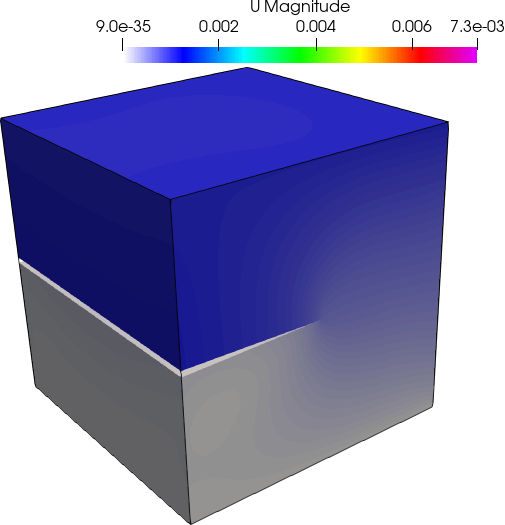
\includegraphics[width=0.24\textwidth]{./Images/u3d0.png}
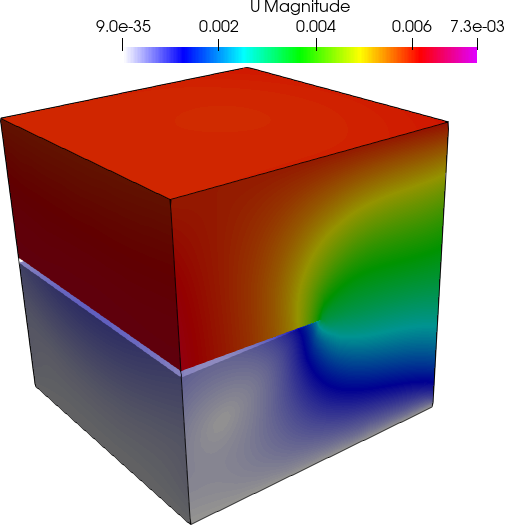
\includegraphics[width=0.24\textwidth]{./Images/u3d1.png}
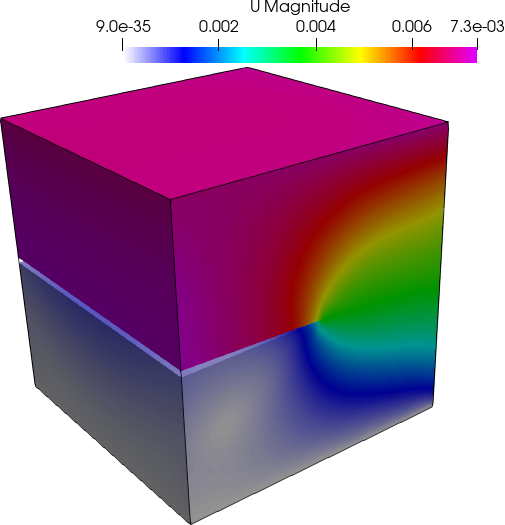
\includegraphics[width=0.24\textwidth]{./Images/u3d2.png}
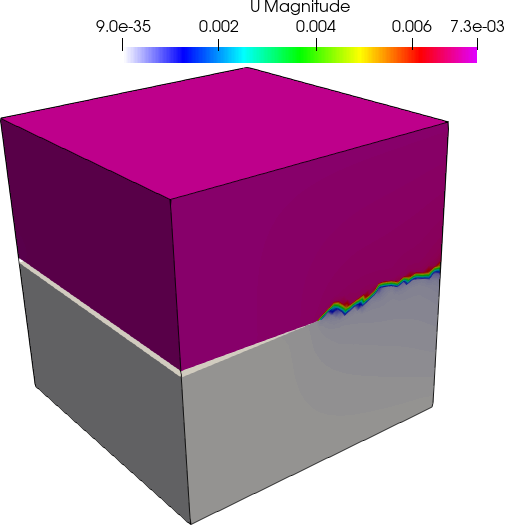
\includegraphics[width=0.24\textwidth]{./Images/u3d3.png}
\caption{Finite element displacement visualised for the 3D problem with ParaView at different timesteps (quasi-statics). Time progresses from left to right in a row and top to bottom when comparing rows. \label{u3d-fem}}
\end{figure}

\begin{figure}[h!]
\centering

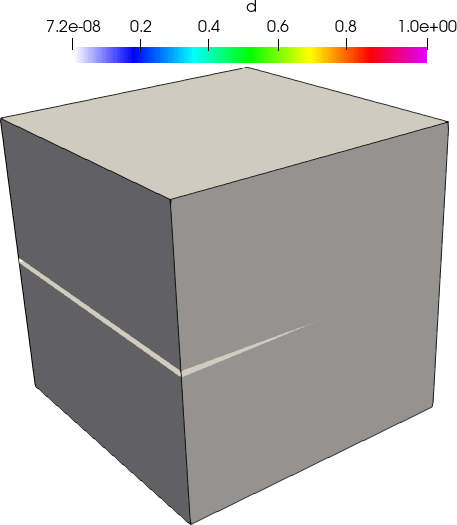
\includegraphics[width=0.24\textwidth]{./Images/d3d0.png}
\includegraphics[width=0.24\textwidth]{./Images/d3d1.png}
\includegraphics[width=0.24\textwidth]{./Images/d3d2.png}
\includegraphics[width=0.24\textwidth]{./Images/d3d3.png}
\caption{Finite element damage visualised for the 3D problem with ParaView at different timesteps (quasi-statics). Time progresses from left to right in a row and top to bottom when comparing rows. \label{d3d-fem}}
\end{figure}

Figures \ref{u3d-fem} and \ref{d3d-fem} present the finite element
displacement and damage field of the 3D problem, which enable us to
visualise the cracking of the cubic specimen.

}



\subsection{Parallel 3D and calculate reactionforce}


{
	\renewcommand{\subsection}{\subsubsection}
	\newcommand{\psd}[1]{{\small\sffamily{\color{blue!60}#1}}}


\subsection{Parallel 2D tensile cracking and calculate-ploting reaction-force}

In solid mechanics often the quantities of interest includes plots such
as reaction-force on a surface vs.~the applied force. Often times these
are experimental outputs and are used for validation.

PSD provides routines to calculate the reaction force on a surface and
also provides means of live plotting (run-time) of these results.
Imagine the test case of tensile cracking of plate (2D) as discussed
above. Considering we are now interested in seeing the plot of reaction
force at surface vs.~the applied tensile displacement, we would need to
use two extra flags in the \psd{ PSD\_PreProcess} step. These flags are
\psd{-getreactionforce} and \psd{ -reactionforce  stress\_based } as
read below:

\begin{lstlisting}[style=BashInputStyle]
PSD_PreProcess -dimension 2 -problem damage -model hybrid_phase_field \
-dirichletconditions 2 -getreactionforce -reactionforce stress_based
\end{lstlisting}

The flag \psd{-getreactionforce} directs PSD to include the routines to
get the reaction force and \psd{ -reactionforce  stress\_based } is the
method by which we get reaction force, in this case reaction force is
calculated using integral of stress in \(y\) direction
\(F_y=\int_{\partial\Omega_{top}} \sigma_y\). Other method
\psd{ -reactionforce variational\_based} also exists within PSD, which
is more accurate but slower, this method calculates reaction force based
on matrix vector multiplication \({F_x,F_y}=\mathbf{A}{u_1,u_2}\) .

Run the problem in the usual way bu using \psd{ PSD\_Solve} and
appropriate number of processes and mesh. While the PSD solver runs it
will create a file \psd{ force.data} that contains the reaction force
and the applied traction.

\begin{lstlisting}[style=BashInputStyle]
PSD_Solve -np 4 Main.edp -mesh ./../Meshes/2D/tensile-crack.msh -v 0
\end{lstlisting}

You can then go ahead and plot \psd{ force.data} to see how \(F_y\) and
\(F_x\) evolve with \(\Delta u_2\). Within the file the first column is
the loading \(\Delta u_2\), the second and the third columns are the
forces \(F_x\) and \(F_y\).

\begin{figure}[h!]
\centering

\includegraphics[width=0.4\textwidth]{./Images/plot-fd.png}
\caption{Applied traction vs. force in y direction. \label{fd-plot}}
\end{figure}

Optionally if you have GnuPlot configured with PSD you can see live
ploting of this curve if you use option \psd{-plotreactionforce} during
the \psd{ PSD\_PreProcess}.

\begin{figure}[h!]
\centering

\includegraphics[width=0.3\textwidth]{./Images/gp0.png}\includegraphics[width=0.3\textwidth]{./Images/gp1.png}\includegraphics[width=0.3\textwidth]{./Images/gp2.png}
\caption{Applied traction vs. force in y direction plotted live using PSD. \label{gnuplot-plot}}
\end{figure}

\textbf{Parallel 3D and calculate reactionforce}

\begin{lstlisting}[style=BashInputStyle]
PSD_PreProcess -dimension 3 -problem damage -model hybrid_phase_field \
-dirichletconditions 2 -getreactionforce -reactionforce stress_based
\end{lstlisting}

\begin{lstlisting}[style=BashInputStyle]
PSD_Solve -np 3 Main.edp -mesh ./../Meshes/3D/tensile-crack.msh -v 0
\end{lstlisting}

}


\subsection{L-shape cracking with point loading}
{
	\renewcommand{\subsection}{\subsubsection}
	\newcommand{\psd}[1]{{\small\sffamily{\color{blue!60}#1}}}

\begin{figure}[h!]
\centering
\includegraphics[width=0.3\textwidth]{./Images/fm-geometry.png}
\caption{Geometry of the L-shaped test used in this tutorial. \label{L-shape-geo}}
\end{figure}

\subsection{Preprocessing}

You can either solver the problem using vectorial approach (recommended)
or using staggered approach. To generate the solver use either from
below.

\textbf{Generation of solver (vectorial)}

\begin{lstlisting}[style=BashInputStyle]
PSD_PreProcess -dimension 2 -problem damage -model hybrid_phase_field \
-dirichletconditions 1 -dirichletpointconditions 1 -debug -postprocess ud \
-energydecomp -constrainHPF -vectorial -getreactionforce -plotreactionforce \
-reactionforce variational_based
\end{lstlisting}

\textbf{Generating solver (staggered)}

\begin{lstlisting}[style=BashInputStyle]
PSD_PreProcess -dimension 2 -problem damage -model hybrid_phase_field \
-dirichletconditions 1 -dirichletpointconditions 1 -debug -postprocess ud \
-energydecomp -constrainHPF -getreactionforce -plotreactionforce \
-reactionforce variational_based
\end{lstlisting}

\subsection{Edit Cycle}

\textbf{Edit ControlParameter.edp:}

\begin{itemize}

\item Update physical parameter, change

\begin{lstlisting}[style=CppStyle]
  real lambda = 121.15e3 ,
       mu     = 80.77e3  ,
       Gc     = 2.7      ;
\end{lstlisting}

to

\begin{lstlisting}[style=CppStyle]
  real lambda = 6.16e3 ,
       mu     = 10.95e3 ,
       Gc     = 8.9e-2  ;
\end{lstlisting}

\item Update solver parameter , change

\begin{lstlisting}[style=CppStyle]
  real lfac  = 2.0  ,
       maxtr = 7e-3 ,
       tr    = 1e-5 ,
       dtr   = 1e-5 ,
       lo           ;
\end{lstlisting}

to

\begin{lstlisting}[style=CppStyle]
  real lfac  = 2.0  ,
       maxtr = 1    ,
       tr    = 1e-2 ,
       dtr   = 1e-2 ,
       lo           ;
\end{lstlisting}


\item Enter the correct Point boundary condition, change

\begin{lstlisting}[style=CppStyle]
  real[int,int] PbcCord = [
//-------------------- [  x  , y  ] --------------------//
                       [  0. , 0. ]    // point 0
//------------------------------------------------------//
                      ];

   macro Pbc0Ux  -0. //
   macro Pbc0Uy  -0. //
\end{lstlisting}

to

\begin{lstlisting}[style=CppStyle]
  real[int,int] PbcCord = [
//-------------------- [  x  , y  ] --------------------//
                       [  470., 250. ]    // point 0
//------------------------------------------------------//
                      ]
;
   macro Pbc0Uy  tr //
\end{lstlisting}

\end{itemize}

\textbf{Edit LinearFormBuilderAndSolver.edp:}

\begin{itemize}

\item To postprocess correct reaction forces in LinearFormBuilderAndSolver.edp for vectorial solver, change

\begin{lstlisting}[style=CppStyle]
  for(int i=0; i < Th.nv; i++){
     if(abs(Th(i).y-1.)<.000001){
        forcetotx = forcetotx + F[][i*3]*DP[i*3];
        forcetoty = forcetoty + F[][i*3+1]*DP[i*3+1];
     }
  }
\end{lstlisting}

to

\begin{lstlisting}[style=CppStyle]
  if(mpirank==mpirankPCi[0]){
     forcetotx = forcetotx + F[][PCi[0]*3+0]*DP[PCi[0]*3+0];
     forcetoty = forcetoty + F[][PCi[0]*3+1]*DP[PCi[0]*3+1];
  }
\end{lstlisting}

\item To postprocess correct reaction forces in LinearFormBuilderAndSolver.edp for staggered solver, change

\begin{lstlisting}[style=CppStyle]
  for(int i=0; i < Th.nv; i++){
     if(abs(Th(i).y-1.)<.000001){
        forcetotx = forcetotx + F[][i*2]*DP[i*2];
        forcetoty = forcetoty + F[][i*2+1]*DP[i*2+1];
     }
  }
\end{lstlisting}

to

\begin{lstlisting}[style=CppStyle]
  if(mpirank==mpirankPCi[0]){
     forcetotx = forcetotx + F[][PCi[0]*2+0]*DP[PCi[0]*2+0];
     forcetoty = forcetoty + F[][PCi[0]*2+1]*DP[PCi[0]*2+1];
  }
\end{lstlisting}

\item Finally to include cyclic loading, change

\begin{lstlisting}[style=CppStyle]
  //-----------------updating traction----------------//

  tr += dtr;
\end{lstlisting}


to

\begin{lstlisting}[style=CppStyle]
  //-----------------updating traction----------------//

  if(iterout<50)
     tr += dtr;
  if(iterout>=51 && iterout<110)
     tr -= dtr;
  if(iterout>=111)
     tr += dtr;
\end{lstlisting}

\begin{figure}[h!]
\centering
\includegraphics[width=0.3\textwidth]{./Images/fm-mesh.png}
\caption{Finite element mesh of the L-shaped test. \label{L-shape-mesh}}
\end{figure}

\end{itemize}

\subsection{Solving}

Irrespective of weather vectorial or staggered mode is used solve the
problem using \psd{PSD\_Solve}

\begin{lstlisting}[style=BashInputStyle]
PSD_Solve -np 4 Main.edp -wg -v 0 -mesh ./../Meshes/2D/L-shaped-crack.msh
\end{lstlisting}

\subsection{Postprocessing}

Use ParaView to post process results.

\begin{figure}[h!]
\centering
\includegraphics[width=0.3\textwidth]{./Images/fm-d1.png}
\includegraphics[width=0.3\textwidth]{./Images/fm-d2.png}
\includegraphics[width=0.3\textwidth]{./Images/fm-d3.png}
\caption{Finite element solution showing: Crack initiation,  movement, and  development. \label{L-shape-mesh-crack}}
\end{figure}

On you screen, the force displacement curve which plots \psd{force.data}
should look something like this

\begin{figure}[h!]
\centering
\includegraphics[width=0.5\textwidth]{./Images/fm-force-displacement.png}
\caption{Force-displacement curve with cyclic loading. \label{L-shape-fd-curve}}
\end{figure}

}

\subsection{Additional exercises on damage}
{
	\renewcommand{\subsection}{\subsubsection}
	\newcommand{\psd}[1]{{\small\sffamily{\color{blue!60}#1}}}

\subsection{Exercise 1}

When calculating the reaction force produced on a surface, optionally
try changing \psd{-reactionforce stress\_based} to
\psd{-reactionforce variational\_based} for changing the method to
extract reaction force, note that stress based method is way faster.

\subsection{Exercise 2}

Optionally try using \psd{-useGFP} flag with \psd{PSD\_PreProcess}
optimized solver. GFP acrynom for GoFast Plugins is a suite of C++ based
fuctions built for PSD that are speed optimal.

\subsection{Exercise 3}

Add \psd{-sequential} flag to \psd{PSD\_PreProcess} for sequential
solver, but remember to use \psd{PSD\_Solve\_Seq} instead of
\psd{PSD\_Solve}

\subsection{Advanced Exercise 1}

try the \psd{-vectorial} flag for vectorial finite element method

\subsection{Advanced Exercise 2}

try the \psd{-energydecomp} flag for using split of tensile energy

\subsection{Advanced Exercise 3}

try using \psd{-constrainHPF} flag for using the constrain condition in
hybrid phase field model

}

\pagebreak

\section{Elastodynamics}

\subsection{Parallel 2D}

{
	\renewcommand{\subsection}{\subsubsection}
	\newcommand{\psd}[1]{{\small\sffamily{\color{blue!60}#1}}}



The problem of interest is a single Dirichlet condition (clamped end
bar) and traction loading. For this example we use Newmark-\(\beta\)
time discretization. Additionally postrocessing is demanded for
displacement, acceleration, and velocity (\(u,a,v\)).

\begin{lstlisting}[style=BashInputStyle]
PSD_PreProcess -dimension 2 -problem elastodynamics -dirichletconditions 1 -tractionconditions 1 \
-timediscretization newmark_beta -postprocess uav
\end{lstlisting}

Once the step above has been performed, we solve the problem using two
MPI processes, with the given mesh file \psd{bar-dynamic.msh}.

\begin{lstlisting}[style=BashInputStyle]
PSD_Solve -np 2 Main.edp -mesh ./../Meshes/2D/bar-dynamic.msh -v 0
\end{lstlisting}

\begin{figure}[h!]
\includegraphics[width=0.19\textwidth]{./Images/ed-u0.png}
\includegraphics[width=0.19\textwidth]{./Images/ed-u2.png}
\includegraphics[width=0.19\textwidth]{./Images/ed-u3.png}
\includegraphics[width=0.19\textwidth]{./Images/ed-u4.png}
\includegraphics[width=0.19\textwidth]{./Images/ed-u5.png}
\caption{Finite element displacement field on warped mesh shown at different time steps. \label{bar-ed}}
\end{figure}

Using ParaView for postprocessing the results that are provided in the
\psd{VTUs...} folder, results such as those shown in
figure\textasciitilde{}\ref{bar-ed} can be extracted.

}

\subsection{Parallel 3D}

{
	\renewcommand{\subsection}{\subsubsection}
	\newcommand{\psd}[1]{{\small\sffamily{\color{blue!60}#1}}}




The problem of interest is a single Dirichlet condition (clamped end
bar) and traction loading. For this example we use Newmark-\(\beta\)
time discretization. Additionally postrocessing is demanded for
displacement, acceleration, and velocity (\(u,a,v\)).

\begin{lstlisting}[style=BashInputStyle]
PSD_PreProcess -dimension 3 -problem elastodynamics -dirichletconditions 1 -tractionconditions 1 \
-timediscretization newmark_beta
\end{lstlisting}

Once the step above has been performed, we solve the problem using four
MPI processes, with the given mesh file \psd{bar-dynamic.msh}.

\begin{lstlisting}[style=BashInputStyle]
PSD_Solve -np 4 Main.edp -mesh ./../Meshes/3D/bar-dynamic.msh -v 0
\end{lstlisting}

}


\subsection{Sequential problems}

{
	\renewcommand{\subsection}{\subsubsection}
	\newcommand{\psd}[1]{{\small\sffamily{\color{blue!60}#1}}}




To the same problems above Add \psd{-sequential} flag to
\psd{PSD\_PreProcess} for sequential solver, but remember to use
\psd{PSD\_Solve\_Seq} instead of \psd{PSD\_Solve}. So the work flow for
the 2D problem would be:

\begin{lstlisting}[style=BashInputStyle]
PSD_PreProcess -dimension 2 -problem elastodynamics -dirichletconditions 1 -tractionconditions 1 \
-timediscretization newmark_beta -postprocess uav -sequential
\end{lstlisting}

Once the step above has been performed, we solve the problem using the
given mesh file \psd{bar-dynamic.msh}.

\begin{lstlisting}[style=BashInputStyle]
PSD_Solve_Seq -np 2 Main.edp -mesh ./../Meshes/2D/bar-dynamic.msh -v 0
\end{lstlisting}

Similarly try out the 3D problem as well.

}

\subsection{Different time discretization}

{
	\renewcommand{\subsection}{\subsubsection}
	\newcommand{\psd}[1]{{\small\sffamily{\color{blue!60}#1}}}



PSD offers different time discretization techniques for solving time
dependent problems. For this example instead of using Newmark-\(\beta\)
time discretization let us switch to more advanced
Generalized-\(\alpha\) one. This can be done by
\psd{-timediscretization generalized\_alpha}, so for example for a 2D
problem we use:

\begin{lstlisting}[style=BashInputStyle]
PSD_PreProcess -dimension 2 -problem elastodynamics -dirichletconditions 1 -tractionconditions 1 \
-timediscretization generalized_alpha -postprocess uav
\end{lstlisting}

Once the step above has been performed, we solve the problem using three
MPI processes, with the given mesh file \psd{bar-dynamic.msh}.

\begin{lstlisting}[style=BashInputStyle]
PSD_Solve -np 3 Main.edp -mesh ./../Meshes/2D/bar-dynamic.msh -v 0
\end{lstlisting}

Similarly try out the 3D problem as well.

}

\subsection{Comparing CPU time}

{
	\renewcommand{\subsection}{\subsubsection}
	\newcommand{\psd}[1]{{\small\sffamily{\color{blue!60}#1}}}


PSD provides mean to time log your solver via \psd{-timelog} flag. What
this will do when you run your solver, on the terminal you will have
information printed on what is the amount of time taken by each step of
your solver. Warning, this will make your solver slower, as this action
involves MPIbarrier routines for correctly timing operation.

An example work flow of 2D solver with timelogging:

\begin{lstlisting}[style=BashInputStyle]
PSD_PreProcess -dimension 2 -problem elastodynamics -dirichletconditions 1 -tractionconditions 1 \
-timediscretization newmark_beta -postprocess uav -timelog
\end{lstlisting}

Once the step above has been performed, we solve the problem using two
MPI processes, with the given mesh file \psd{bar-dynamic.msh}.

\begin{lstlisting}[style=BashInputStyle]
PSD_Solve -np 2 Main.edp -mesh ./../Meshes/2D/bar-dynamic.msh -v 0
\end{lstlisting}

\begin{figure}[h!]
\centering
\includegraphics[width=0.4\textwidth]{./Images/ed-time-par.png}
\caption{Time logging output produced for parallel run on 2 processes.\label{time-par-ed}}
\end{figure}

The figure\textasciitilde{}\ref{time-par-ed} shows the time logging
output produced for parallel run on 2 processes using \psd{-timelog}
flag. Similar output is produced for sequential solver of the same
problem shown in figure\textasciitilde{}\ref{time-seq-ed}. Take note of
the speed up, which should be two folds - parallel solver solves the
full problem in half the time (1.5 sec) than that of sequential solver
(3.3 sec). This is due to the fact we used 2 MPI processes.

Also take note of timings produced for different operations of the
solver. Note that in figures\textasciitilde{}\ref{time-par-ed},
\ref{time-seq-ed}, we only see the final time step of the solved
problem.

\begin{figure}[h!]
\centering
\includegraphics[width=0.4\textwidth]{./Images/ed-time-seq.png}
\caption{Time logging output produced for parallel run on 2 processes.\label{time-seq-ed}}
\end{figure}

}

\subsection{Additional exercises on damage}
{
	\renewcommand{\subsection}{\subsubsection}
	\newcommand{\psd}[1]{{\small\sffamily{\color{blue!60}#1}}}


\subsection{Exercise 1}

You are encouraged to try out timelogging and find out if the code
(parallel/sequential) is any faster when we use Newmark-\(\beta\) or
Generalized-\(\alpha\). Read the documentation for other types of time
discretizations that can be performed with PSD, try each one out with
\psd{-timelog} and compare.

\subsection{Exercise  2}

There is a solver run level flag for mesh refinement
\footnote{Mesh refinement is performed after partitioning.}. This flag
is called \psd{-split [int]} which splits the triangles (resp.
tetrahedrons) of your mesh into four smaller triangles (resp.
tetrahedrons). As such \psd{-split 2} will produce a mesh with 4 times
the elements of the input mesh. Similarly, \psd{-split n} where \(n\) is
a positive integer produces \(2^n\) times more elements than the input
mesh. You are encouraged to use this \psd{-split} flag to produce
refined meshes and check, mesh convergence of a problem, computational
time, etc. Use of parallel computing is recommended. You could try it
out with \psd{PSD\_Solve} or \psd{PSD\_Solve\_Seq}, for example:

\begin{lstlisting}[style=BashInputStyle]
PSD_Solve -np 2 Main.edp -mesh ./../Meshes/2D/bar-dynamic.msh -v 0 -split 2
\end{lstlisting}

for splitting each triangle of the mesh \psd{bar-dynamic.msh} into 4.

\subsection{Exercise  3}

There is a preprocess level flag \psd{-debug}, which as the name
suggests should be used for debug proposes by developers. However, this
flag will activate OpebGL live plotting of the problem, with displaced
mesh. You are encouraged to try it out

\begin{lstlisting}[style=BashInputStyle]
PSD_PreProcess -dimension 2 -problem elastodynamics -dirichletconditions 1 -tractionconditions 1 \
-timediscretization newmark_beta -postprocess uav -timelog -debug
\end{lstlisting}

Then to run the problem we need aditional \psd{-wg} flag

\begin{lstlisting}[style=BashInputStyle]
PSD_Solve -np 2 Main.edp -mesh ./../Meshes/2D/bar-dynamic.msh -v 0 -wg
\end{lstlisting}

\subsection{Exercise  4}

PSD comes with additional set of plugins/functions that are highly
optimized for performing certain operations during solving. These
operations are handled by GoFast Plugins (GFP) kernel of PSD (optimize
C++ classes/templates/structures), by default this functionality is
turned off and not used. You are encouraged to try out using GFP
functions in a solver by using \psd{-useGFP} flag flag to
\psd{PSD\_PreProcess} For example, the PSD solver workflow for the first
2D example in this tutorial would be:

\begin{lstlisting}[style=BashInputStyle]
PSD_PreProcess -dimension 2 -problem elastodynamics -dirichletconditions 1 -tractionconditions 1 \
-timediscretization newmark_beta -postprocess uav -useGFP
\end{lstlisting}

Once the step above has been performed, we solve the problem using, with
the given mesh file \psd{bar-dynamic}.

\begin{lstlisting}[style=BashInputStyle]
PSD_Solve -np 2 Main.edp -mesh ./../Meshes/2D/bar-dynamic.msh -v 0 -wg
\end{lstlisting}

Try it out for other problems of this tutorial. \psd{-useGFP} should
lead to a faster solver, it might be a good idea to always use this
option. To go one step further, use \psd{-timelog} flag and determine if
you have some speed up.

}


\pagebreak

\section{Soil dynamics}

{
	\renewcommand{\subsection}{\subsubsection}
	\newcommand{\psd}[1]{{\small\sffamily{\color{blue!60}#1}}}


The problem of interest is a single Dirichlet condition problem of
soildynamics in 2D. For this problem we use Newmark-\(\beta\) time
discretization. Additionally postrocessing is demanded for displacement,
acceleration, and velocity (\(u,a,v\)).

\begin{lstlisting}[style=BashInputStyle]
PSD_PreProcess -dimension 2 -problem soildynamics -dirichletconditions 1 -timediscretization newmark_beta \
-postprocess uav
\end{lstlisting}

Once the step above has been performed, we solve the problem using four
MPI processes, with the given mesh file \psd{soil.msh}.

\begin{lstlisting}[style=BashInputStyle]
PSD_Solve -np 4 Main.edp -mesh ./../Meshes/2D/soil.msh -v 0
\end{lstlisting}

\begin{figure}[h!]
\centering
\includegraphics[width=0.4\textwidth]{./Images/sd-u0.png}
\includegraphics[width=0.4\textwidth]{./Images/sd-u1.png}\\
\includegraphics[width=0.4\textwidth]{./Images/sd-u2.png}
\includegraphics[width=0.4\textwidth]{./Images/sd-u3.png}\\
\includegraphics[width=0.4\textwidth]{./Images/sd-u4.png}
\caption{Finite element displacement and velocity fields visualized for the 2D problem with ParaView at different timesteps. \label{bar-sd}}
\end{figure}

Using ParaView for postprocessing the results that are provided in the
\psd{VTUs...} folder, results such as those shown in
figure\textasciitilde{}\ref{bar-sd} can be extracted.

}


\subsection{Parallel 3D}

{
	\renewcommand{\subsection}{\subsubsection}
	\newcommand{\psd}[1]{{\small\sffamily{\color{blue!60}#1}}}



The problem of interest is a single Dirichlet condition problem of
soildynamics in 3D. For this problem we use Newmark-\(\beta\) time
discretization. Additionally postrocessing is demanded for displacement,
acceleration, and velocity (\(u,a,v\)).

\begin{lstlisting}[style=BashInputStyle]
PSD_PreProcess -dimension 3 -problem soildynamics -dirichletconditions 1 -timediscretization newmark_beta \
-postprocess uav
\end{lstlisting}

Once the step above has been performed, we solve the problem using three
MPI processes, with the given mesh file \psd{soil.msh}.

\begin{lstlisting}[style=BashInputStyle]
PSD_Solve -np 3 Main.edp -mesh ./../Meshes/3D/soil.msh -v 0
\end{lstlisting}

\begin{figure}[h!]
\centering
\includegraphics[width=0.4\textwidth]{./Images/sd-3du0.png}
\includegraphics[width=0.4\textwidth]{./Images/sd-3du1.png}\\
\includegraphics[width=0.4\textwidth]{./Images/sd-3du2.png}
\includegraphics[width=0.4\textwidth]{./Images/sd-3du3.png}\\
\includegraphics[width=0.4\textwidth]{./Images/sd-3du4.png}
\caption{Finite element displacement and velocity fields visualized for the 3D problem with ParaView at different timesteps. \label{bar3d-sd}}
\end{figure}

Using ParaView for postprocessing the results that are provided in the
\psd{VTUs...} folder, results such as those shown in
figure\textasciitilde{}\ref{bar3d-sd} can be extracted.

}

\subsection{Parallel 2D with double couple}

{
	\renewcommand{\subsection}{\subsubsection}
	\newcommand{\psd}[1]{{\small\sffamily{\color{blue!60}#1}}}





In the 2D problem above seismic sources was supplied on the border, in
the current one the source is more realistic and comes from a double
couple (point Dirichlet condition). The double couple boundary condition
is a way to impose moments caused by faults that create earthquakes,
here in this problem double couple is imposed using displacement based.

\begin{lstlisting}[style=BashInputStyle]
PSD_PreProcess -dimension 2 -problem soildynamics -model linear -timediscretization newmark-beta \
-useGFP -doublecouple displacement-based -postprocess uav
\end{lstlisting}

Once the step above has been performed, we solve the problem using two
MPI processes, with the given mesh file \psd{soil-dc.msh}.

\begin{lstlisting}[style=BashInputStyle]
PSD_Solve -np 2 Main.edp -v 1 -ns -nw -mesh ./../Meshes/2D/soil-dc.msh
\end{lstlisting}

\begin{figure}[h!]
\centering
\includegraphics[width=0.45\textwidth]{./Images/sd-2ddcu0.png}
\includegraphics[width=0.45\textwidth]{./Images/sd-2ddcu1.png}\\
\includegraphics[width=0.45\textwidth]{./Images/sd-2ddcu2.png}
\caption{Finite element displacement and acceleration fields visualized for the 2D problem with ParaView at different timesteps. \label{bar2ddc-sd}}
\end{figure}

Using ParaView for postprocessing the results that are provided in the
\psd{VTUs...} folder, results such as those shown in
figure\textasciitilde{}\ref{bar2ddc-sd} can be extracted.

Similarly try out the 3D problem. However take note that a the mesh
\psd{./../Meshes/2D/soil-dc.msh} is not provided, so you will have to
create your own mesh.

}
\subsection{Parallel 3D with top-ii-vol meshing}

{
	\renewcommand{\subsection}{\subsubsection}
	\newcommand{\psd}[1]{{\small\sffamily{\color{blue!60}#1}}}


Single Dirichlet at the bottom and using GFP.

\begin{lstlisting}[style=BashInputStyle]
PSD_PreProcess -dimension 3 -problem soildynamics -model linear -timediscretization newmark_beta \
-useGFP -top2vol-meshing -timediscretization newmark-beta -postprocess uav
\end{lstlisting}

\begin{lstlisting}[style=BashInputStyle]
PSD_Solve -np 4 Main.edp -v 0 -ns -nw 
\end{lstlisting}

}


\subsection{Parallel 3D with top-ii-vol meshing and double couple source}

{
	\renewcommand{\subsection}{\subsubsection}
	\newcommand{\psd}[1]{{\small\sffamily{\color{blue!60}#1}}}


Single Dirichlet via double couple and using GFP. Double couple is
displacement based.

\begin{lstlisting}[style=BashInputStyle]
PSD_PreProcess -dimension 3 -problem soildynamics -timediscretization newmark_beta \
-useGFP -top2vol-meshing -doublecouple displacement_based -postprocess uav
\end{lstlisting}

\begin{lstlisting}[style=BashInputStyle]
PSD_Solve -np 3 Main.edp -v 0 -ns -nw 
\end{lstlisting}

}

\subsection{Additional exercises on soildynamics}
{
	\renewcommand{\subsection}{\subsubsection}
	\newcommand{\psd}[1]{{\small\sffamily{\color{blue!60}#1}}}

\subsection{Exercise  1}

You are encouraged to try out sequential PSD solver, to do so used add
\psd{-sequential} flag to \psd{PSD\_PreProcess} step and run the solver
with \psd{PSD\_Solve\_Seq} instead of \psd{PSD\_Solve}. For example, the
PSD sequential solver workflow for the first 2D example in this tutorial
would be:

\begin{lstlisting}[style=BashInputStyle]
PSD_PreProcess -dimension 2 -problem soildynamics -dirichletconditions 1 -timediscretization newmark_beta \
-postprocess uav -sequential
\end{lstlisting}

Once the step above has been performed, we solve the problem using
\psd{PSD\_Solve\_Seq}, with the given mesh file \psd{soil.msh}.

\begin{lstlisting}[style=BashInputStyle]
PSD_Solve_Seq  Main.edp -mesh ./../Meshes/2D/soil.msh -v 0
\end{lstlisting}

Try it out for other problems of this tutorial.

\subsection{Exercise 2}

For soildynamic problems with double couple source, the double couple
source can be introduced into the solver either by displacement-based
operator -- providing displacements at the double couple points that
will be converted to moments -- or by force-based operators -- providing
forces at the double couple points that will be converted to moments. In
the tutorials above we already tried displacement-based way of
introducing double couple source by using
\psd{-doublecouple displacement\_based}. You are encouraged to try out
the force-based double couple source by using
\psd{-doublecouple force\_based}.

\subsection{Exercise 3}

You are encouraged to try out timelogging and find out if the code
(parallel/sequential) is any faster when we use Newmark-\(\beta\) or
Generalized-\(\alpha\). Read the documentation for other types of time
discretizations that can be performed with PSD, try each one out with
\psd{-timelog} and compare.

\subsection{Exercise  4}

PSD comes with additional set of plugins/functions that are highly
optimized for performing certain operations during solving. These
operations are handled by GoFast Plugins (GFP) kernel of PSD (optimize
C++ classes/templates/structures), by default this functionality is
turned off and not used. You are encouraged to try out using GFP
functions in a solver by using \psd{-useGFP} flag flag to
\psd{PSD\_PreProcess} For example, the PSD solver workflow for the first
2D example in this tutorial would be:

\begin{lstlisting}[style=BashInputStyle]
PSD_PreProcess -dimension 2 -problem soildynamics -dirichletconditions 1 -timediscretization newmark\_beta \
-postprocess uav -useGFP
\end{lstlisting}

Once the step above has been performed, we solve the problem using, with
the given mesh file \psd{soil.msh}.

\begin{lstlisting}[style=BashInputStyle]
PSD_Solve -np 4 Main.edp -mesh ./../Meshes/2D/soil.msh -v 0
\end{lstlisting}

Try it out for other problems of this tutorial. \psd{-useGFP} should
lead to a faster solver, it might be a good idea to always use this
option. To go one step further, use \psd{-timelog} flag and determine if
you have some speed up.

}

\section{Elasto Plasticity}

\subsection{Elastoplacity using PSD-MFront interface}
{
	\renewcommand{\subsection}{\subsubsection}
	\newcommand{\psd}[1]{{\small\sffamily{\color{blue!60}#1}}}

\section{Introduction}

This tutorial is concerned with a non-linear problem of the incremental
analysis of an elasto-plastic Von-Mises material. A two-dimensional test
(in \(x-y\)) will be considered. The problem of interest is a quarter of
a cylinder (with external radius \(R_e\) and internal radius \(R_i\))
\cref{bar-sd}. Boundary conditions correspond to symmetry conditions on
the bottom horizontal \(y=0\) and left vertical borders \(x=0\) (resp.
numbered 1 and 3 as mesh labels). Loading consists of a uniform pressure
(traction boundary) on the internal boundary (numbered 4 as mesh label).
Load (pressure) \(q\) will be progressively increased from 0 to
\(q_{\text{lim}}=\frac{2}{\sqrt3}\sigma_0\text{log}(\frac{R_e}{R_i})\)
which is the analytical collapse load for a perfectly-plastic material
(no hardening):

\begin{figure}[h!]
\centering
\includegraphics[width=0.3\textwidth]{./Images/nl-arc.png}
\caption{Domain of the non-linear problem. \label{bar-sd}}
\end{figure}

The material is represented by an isotropic elasto-plastic von Mises
yield condition of uniaxial strength \(\sigma_0\) and with isotropic
hardening of modulus \(H\). The yield condition is thus given by:

\[f(\sigma)=\sqrt{\frac{3}{2}s:s}-\sigma_0-Hp\le0\]

where \(p\) is the cumulated equivalent plastic strain and \(s\)
denoting the deviatoric elastic stress
\(s = \text{dev} \sigma_{\text{elas}}\). The hardening modulus can also
be related to a tangent elastic modulus \(E_t=\frac{EH}{E+H}\).

To compute the structures response an iterative predictor-corrector
return mapping algorithm embedded in a Newton-Raphson global loop for
restoring equilibrium is used. Due to the simple expression of the von
Mises criterion, the return mapping procedure is completely analytical
(with linear isotropic hardening). We point out that the two-dimensional
nature of the problem will be impose keeping track of the out-of-plane
\(\varepsilon^p_{zz}\) plastic strain and dealing with representations
of stress/strain states including the \(zz\) component.

The displacement field evolution during the cylinder expansion will look
like this the one presented in \cref{bar-sd}:

\begin{figure}[h!]
\centering
\includegraphics[width=0.3\textwidth]{./Images/nl-ep-t0.png}\includegraphics[width=0.3\textwidth]{./Images/nl-ep-t4.png}\includegraphics[width=0.3\textwidth]{./Images/nl-ep-t8.png}\\
\includegraphics[width=0.3\textwidth]{./Images/nl-ep-t12.png}\includegraphics[width=0.3\textwidth]{./Images/nl-ep-t16.png}\includegraphics[width=0.3\textwidth]{./Images/nl-ep-t19.png}
\caption{Warped displacement field evolution - from top left $t_0,t_4,t_8,t_{12},t_{16},t_{19}$. \label{bar-sd}}
\end{figure}

The return mapping procedure consists in finding a new stress
\(\sigma_{n+1}\) and internal variable \(p_{n+1}\) state verifying the
current plasticity condition from a previous stress \(\sigma_n\) and
internal variable \(p_{n}\) state and an increment of total deformation
\(\Delta \varepsilon\). All this is handled by MFront, where MFront
requests PSD for the previous \(n\) time-step strains \(\varepsilon_n\).
In order to use a Newton-Raphson procedure to resolve global
equilibrium, we also need to derive the algorithmic consistent tangent
matrix which is also given by MFront.

Within MFront an elastic trial stress
\(\sigma_{\text{elas}} = \sigma_{n} + \mathbf{M}\Delta \varepsilon\) is
first computed. Then the plasticity criterion is then evaluated with the
previous plastic strain
\(f_{\text{elas}}=\sigma_{\text{elas}}^{\text{eq}} - \sigma_0 - Hp_n\),
where \(\sigma_{\text{elas}}^{\text{eq}}=\sqrt{\frac{3}{2}s:s}\).
Consequently, if \(f_{\text{elas}} \le 0\) no plasticity occurs during
this time increment and \(\Delta \varepsilon^p = \Delta p =0\).
Otherwise if \(f_{\text{elas}} > 0\), plasticity occurs and the
increment of plastic strain is given by
\[\Delta p = \frac{f_{\text{elas}}}{3\mu + H}\]

The final stress state is corrected by the plastic strain as follows

\[\sigma_{n+1} = \sigma_{\text{elas}} - \beta s \quad \text{with} \quad \beta=\frac{3\mu}{\sigma_{\text{elas}}^{\text{eq}}}\Delta p\]

\section{Procedure to simulate in PSD}

\subsection{Step 1: Preprocessing}

First step in a PSD simulation is PSD preprocessing, at this step you
tell PSD what kind of physics, boundary conditions, approximations,
mesh, etc are you expecting to solve. More importantly for this tutorial
we will signify to PSD that MFront has to be used.

In the terminal \psd{cd} to the folder
\psd{/home/PSD-tutorials/elasto-plastic}. Launch \psd{PSD\_PreProcess}
from the terminal, to do so run the following command.

\begin{lstlisting}[style=BashInputStyle]
PSD_PreProcess -problem elasto_plastic -model von_mises -dimension 2 \
-tractionconditions 1  -dirichletconditions 2 -postprocess u -useMfront
\end{lstlisting}

After the \psd{PSD\_PreProcess} runs successfully you should see many
\psd{.edp} files in your current folder.

\textbf{What do the arguments mean ?}

\begin{itemize}
\item \psd{-problem elasto\_plastic} means that we are solving elasto plastic problem;
\item \psd{-model von\_mises} means that we are using Von Mises hypothesis;
\item \psd{-dimension 2} means it is a 2D simulation;
\item \psd{-tractionconditions 1} with applied traction force acting on the domain border (pressure);
\item \psd{-dirichletconditions 2} says we have two Dirichlet border;
\item \psd{-postprocess u} means we would like to have ParaView post processing files.
\item \psd{-useMfront} activates MFront interface for PSD.
\end{itemize}

At this stage the input properties \(E,\nu, \sigma_0, E_t, H\) ,
Geometric parameters (internal/external radius of shell) \(R_i, R_e\),
and limiting pressure \(Q_{\text{lim}}\) can be mentioned in
\psd{ControlParameters.edp}. Some of these properties will be shared
with MFront. Have a look at the below given snippet from the file
\psd{ControlParameters.edp}

\begin{lstlisting}[style=CppStyle]
//============================================================================
//                   ------- Material parameters -------                      
// -------------------------------------------------------------------        
//  E, nu : Modulus of Elasticity and Poisson ratio of the material           
//  sig0  : Yield strength of the material                                    
//  Et    : Tangent modulus of the material                                   
//  H     : Hardening modulus of the material                                 
//  PropertyNames : String of material property names (space seperated)       
//                  that are provided to Mfront.                              
//  PropertyValues : Values of material properties provided to Mfront         
//                                                                            
// -------------------------------------------------------------------        
//  NOTE:     Please note that PropertyNames should be the same as            
//            as in the Elasticity.mfront file                                
// -------------------------------------------------------------------        
//============================================================================
                                                                              
  real E    = 70.e3       ,                                                   
       nu   = 0.3         ,                                                   
       sig0 = 250.        ,                                                   
       Et   = E/100.      ,                                                   
       H    = E*Et/(E-Et) ;                                                   
                                                                              
                                                                              
  real Re   = 1.3         ,  // external radius geometry                      
       Ri   = 1.0         ;  // internal radius geometry                      
                                                                              
                                                                              
  real Qlim = 2./sqrt(3.)*log(Re/Ri)*sig0; //  Limiting pressure 
\end{lstlisting}

We then move on to defining the MFront parameters. We, create variables
that can be exchanged with MFront and inform MFront that we would like
to use IsotropicLinearHardeningPlasticity model with PLAINSTRAIN
hypothesis (since we are in 2D) and the given properties. Have a look at
the below given snippet from the file \psd{ControlParameters.edp}

\begin{lstlisting}[style=CppStyle]
  string    MaterialBehaviour   = "IsotropicLinearHardeningPlasticity";     
  string    MaterialHypothesis  = "PLANESTRAIN";                 
  string    PropertyNames       = "YoungModulus PoissonRatio HardeningSlope YieldStrength";
  real[int] PropertyValues      = [ E, nu , H, sig0 ];
\end{lstlisting}

The algorithmic parameters will be set up next, i.e, we signify the
Newton-Raphsons convergence criteria, Newton-Raphsons maximum
iterations, and number of time steps for quasi-time discretization. Have
a look at the below given snippet from the file
\psd{ControlParameters.edp}

\begin{lstlisting}[style=CppStyle]
//============================================================================
//                   ------- Algorithmic parameters -------                   
// -------------------------------------------------------------------        
//  NrEpsCon : Newton-Raphsons Convergence epsilon                            
//  NrMaxItr : Newton-Raphsons maximum iterations                             
//  TlMaxItr : Number of time steps for quasi-time discretization             
//                                                                            
// -------------------------------------------------------------------        
//  NOTE:     Please note that PropertyNames should be the same as            
//            as in the Elasticity.mfront file                                
// -------------------------------------------------------------------        
//============================================================================
                                                                              
  macro EpsNrCon  ()   1.e-8       //                                         
  macro NrMaxItr  ()   200         //                                         
  macro TlMaxItr  ()   20          // 
\end{lstlisting}

Next we notify PSD about the Dirichlet conditions since two Dirichlet
conditions exists we need to provide info about these in. To provide the
\(y\) constained boundary condition (border of the cylinder on
\(x\)-axis) the variables \psd{Dbc0On 1}, \psd{Dbc0Uy 0.}, which means
for Dirichlet border \psd{1} (\psd{Dbc0On 1}) where \psd{1} is the
constrained in \(y\) direction label of the mesh Dirichlet constrain is
applied \psd{Dbc0Uy 0} i.e., the clamped end condition (for
\(\partial\Omega_{\text{meshLabel==1}}\) \(u_y=0\)). Similarly the
Dirichlet constrain is set on vertical border (border of the cylinder on
\(y\)-axis), where \(\partial\Omega_{\text{meshLabel==3}}\) \(u_x=0\).
Have a look at the below given snippet from the file
\psd{ControlParameters.edp}

\begin{lstlisting}[style=CppStyle]
//============================================================================
//        ------- Dirichlet boundary-condition parameters -------             
// ---------------------------------------------------------------------------
// Dbc       : acronym for Dirichlet boundary condition                       
// Dbc(I)On  : is/are the  surface labels tags (integer list) on to which     
//             Dirichlet boundary conditions is to be applied.                
// Dbc(I)Ux  : is the x component of Dirichlet displacement on the surface    
//             border (I) denoted by label(s) Dbc(I)On in the mesh.           
// -------------------------------------------------------------------------- 
// NOTE: either macro Dbc(I)Ux or Dbc(I)Uy or Dbc(I)Uz should  be commented   
//       or deleted if the user does not wish to apply Dirichlet  condition   
//       on that particular  direction (let it free)                          
//============================================================================
                                                                              
  macro  Dbc0On 1   //                            
  macro  Dbc0Uy 0.  //                                               
  macro  Dbc1On 3   //                            
  macro  Dbc1Ux 0.  // 
\end{lstlisting}

Next we set up the traction (pressure) conditions. Have a look at the
below given snippet from the file \psd{ControlParameters.edp}

\begin{lstlisting}[style=CppStyle]
//============================================================================
// ------- Neumann/traction boundary-condition parameters -------             
// ---------------------------------------------------------------------------
// Tbc       : acronym for traction boundary condition                        
// Tbc(I)On  : is/are the  surface labels tags (integer list) on to which     
//             traction boundary conditions is to be applied.                 
// Tbc(I)Tx  : is the x component of traction forces on the surface           
//             border (I) denoted by label(s) Tb(I)On in the mesh.            
// -------------------------------------------------------------------------- 
// NOTE: either macro Tbc(I)Tx or Tbc(I)Ty or Tbc(I)Tz should  be commented   
//       or deleted  if  the  user  does not wish to apply traction on that   
//       particular  direction (let it free)                                  
//============================================================================
                                                                              
  real tl;       // Traction load to be updated in time loop                
  macro  Tbc0On  4           //                                      
  macro  Tbc0Tx  Qlim*tl*N.x //                                      
  macro  Tbc0Ty  Qlim*tl*N.y //  
\end{lstlisting}

Here we use a variable \psd{tl} that will be updated at each time-step.
We signify the traction border \(\partial\Omega_{\text{meshLabel==4}}\)
\(u_x=Q_{\text{lim}}t_lN_x\) and \(u_y=Q_{\text{lim}}t_lN_y\).

\subsection{Step 2: Solving}

As PSD is a parallel solver, let us use 4 cores to solve the 2D bar
case. To do so enter the following command:

\begin{lstlisting}[style=BashInputStyle]
PSD_Solve -np 4 Main.edp -mesh ./../Meshes/2D/quater_cylinder.msh -v 0
\end{lstlisting}

Here \psd{-np 4} denote the argument used to enter the number of
parallel processes (MPI processes) used while solving.
\psd{-mesh ./../Meshes/2D/quater\_cylinder.msh} is used to provide the
mesh file to the solver. \psd{-v 0} denotes the verbosity level on
screen. \psd{PSD\_Solve} is a wrapper around \psd{FreeFem++-mpi}. Note
that if your problem is large use more cores. PSD has been tested upto
13,000 parallel processes and problem sizes with billions of unknowns,
surely you will now need that many for this 2D problem.

\subsection{Step 3: Postprocessing}

PSD allows postprocessing of results in ParaView. After the step 2
mentioned above finishes. Launch ParaView and have a look at the
\psd{.pvd} file in the \psd{VTUs...} folder. Using ParaView for
postprocessing the results that are provided in the \psd{VTUs...}
folder, results such as those shown in \cref{comp2} left column can be
extracted.

\begin{figure}[h!]
\centering
\fbox{\includegraphics[width=0.45\textwidth]{./Images/test_psd_t0.png}}\hspace{1mm}\fbox{\includegraphics[width=0.456\textwidth]{./Images/test_fenics_t0.png}}\vspace{1mm}
\fbox{\includegraphics[width=0.45\textwidth]{./Images/test_psd_t10.png}}\hspace{1mm}\fbox{\includegraphics[width=0.456\textwidth]{./Images/test_fenics_t10.png}}\vspace{1mm}
\fbox{\includegraphics[width=0.45\textwidth]{./Images/test_psd_t19.png}}\hspace{1mm}\fbox{\includegraphics[width=0.456\textwidth]{./Images/test_fenics_t19.png}}\vspace{1mm}
\caption{Validation results comparison of PSD (left column) and reference code (right column) at different timesteps ($t_0, t_{10}, t_{19}$). Reference results used for comparison  were obtained by installing and running the FEniCS Solid Mechanics library [Garth N. Wells (2021)]. \label{comp2}}
\end{figure}

You are all done with your 2D elasto-plastic simulation with Mfront
interface.

\section{Validation}

To thoroughly validate PSD-MFront model and interface, the results
obtained from this tutorial can directly be compared to the ones
observed by (Garth N. Wells 2021). (Garth N. Wells 2021) present a
non-linear solid mechanics solver using the open-source FEniCS library.
Elasto-plastic von Mises material from the (Garth N. Wells 2021) solver
is compared in \cref{comp2,comp1,comp3}. The comparisons match with a
good order of accuracy.

\begin{figure}[h!] 
\centering
\includegraphics[width=0.45\textwidth]{./Images/final.png}
\caption{Validation of the displacement  movement of inner border movement obtained by PSD and another reference code.  Reference results used for comparison  were obtained by installing and running the FEniCS solid mechanics codes \url{https://bitbucket.org/fenics-apps/fenics-solid-mechanics}. \label{comp3}}
\end{figure}

\begin{figure}[h!]
\centering
\includegraphics[width=0.45\textwidth]{./Images/t5.png}\includegraphics[width=0.45\textwidth]{./Images/t19.png}
\caption{Validation of the displacement field obtained by PSD and another reference code. The displacement magnitude is plotted on the central line which bisects the geometry into two. On the left time steps - $t_0,t_4,t_8,t_{12},t_{16}$ are plotted and on the right $t_{19}$. Reference results used for comparison  were obtained by installing and running the FEniCS Solid Mechanics library [Garth N. Wells (2021)]. \label{comp1}}
\end{figure}

\section*{Bibliography}\label{bibliography}
\addcontentsline{toc}{section}{Bibliography}

\hypertarget{refs}{}
\hypertarget{ref-Fenics}{}
Garth N. Wells, Kristian B. Ølgaard. 2021. ``FEniCS Solid Mechanics
library.''
\url{https://bitbucket.org/fenics-apps/fenics-solid-mechanics/src/master/}.

}

\pagebreak

\section{General list of examples: Linear Elasticity}
 *============================================================*\\
  \textbf{Sequential  2D linear-elasticity}\\                   
 *============================================================*\\
\begin{lstlisting}[style=BashInputStyle] 
PSD_PreProcess -dimension 2 -bodyforceconditions 1 conditions 1 -sequential -dirichletconditions 1 
	
PSD_Solve_Seq Main.edp -v 0 -ns -nw 
\end{lstlisting}


*============================================================*\\
 \textbf{Sequential  3D linear-elasticity}                   \\
*============================================================*\\
\begin{lstlisting}[style=BashInputStyle] 
PSD_PreProcess -dimension 3 -bodyforceconditions 1 -sequential -dirichletconditions 1

PSD_Solve_Seq Main.edp -v 0 -ns -nw
\end{lstlisting}


*============================================================*\\
\textbf{ Sequential  2D linear-elasticity fastmethod }      \\
*============================================================*\\
\begin{lstlisting}[style=BashInputStyle] 
PSD_PreProcess -dimension 2 -bodyforceconditions 1 -sequential -dirichletconditions 1 -fastmethod 

PSD_Solve_Seq Main.edp -v 0 -ns -nw	
\end{lstlisting}
*============================================================*\\
\textbf{ Sequential  3D linear-elasticity   fastmethod }     \\
*============================================================*\\
\begin{lstlisting}[style=BashInputStyle] 
PSD_PreProcess -dimension 3 -bodyforceconditions 1 -sequential -dirichletconditions 1 -fastmethod 

PSD_Solve_Seq Main.edp -v 0 -ns -nw  	
\end{lstlisting}



*============================================================*\\
\textbf{ Parallel 2D linear-elasticity }                  \\
*============================================================*\\
	
\begin{lstlisting}[style=BashInputStyle]
PSD_PreProcess -dimension 2 -bodyforceconditions 1  -dirichletconditions 1 

ff-mpirun-np 2  Main.edp -v 0 -ns -nw
\end{lstlisting}
*============================================================\\
\textbf{ Parallel 3D linear-elasticity  }                 \\
*============================================================\\
	
\begin{lstlisting}[style=BashInputStyle]
PSD_PreProcess -dimension 3 -bodyforceconditions 1  -dirichletconditions 1 

ff-mpirun-np 2  Main.edp -v 0 -ns -nw
\end{lstlisting}
*============================================================\\
\textbf{ Parallel 2D linear-elasticity     fastmethod  }            \\
*============================================================\\
	
\begin{lstlisting}[style=BashInputStyle]
PSD_PreProcess -dimension 2 -bodyforceconditions 1  -dirichletconditions 1 -fastmethod  

ff-mpirun-np 2  Main.edp -v 0 -ns -nw	
\end{lstlisting}
*============================================================\\
\textbf{ Parallel 3D linear-elasticity     fastmethod }             \\
*============================================================\\
	
\begin{lstlisting}[style=BashInputStyle]
PSD_PreProcess -dimension 3 -bodyforceconditions 1  -dirichletconditions 1 -fastmethod  

ff-mpirun-np 2  Main.edp -v 0 -ns -nw
\end{lstlisting}

\section{General list of examples: Fracture mechanics}

*============================================================\\
\textbf{ Sequential  2D phase-field fracture mechanics }\\
*============================================================\\
\begin{lstlisting}[style=BashInputStyle]
PSD_PreProcess -dimension 2 -problem damage -model hybrid-phase-field -sequential -dirichletconditions 2   

PSD_Solve Main.edp -v 0 -ns -nw   
\end{lstlisting}
*============================================================\\
\textbf{ Sequential  3D phase-field fracture mechanics}\\ 
*============================================================\\

\begin{lstlisting}[style=BashInputStyle]
PSD_PreProcess -dimension 3 -problem damage -model hybrid-phase-field -sequential -dirichletconditions 2   

PSD_Solve Main.edp -v 0 -ns -nw   
\end{lstlisting}
*============================================================\\
\textbf{ Parallel 2D phase-field fracture mechanics} \\
*============================================================\\

\begin{lstlisting}[style=BashInputStyle]
PSD_PreProcess -dimension 2 -problem damage -model hybrid-phase-field -dirichletconditions 2   

PSD_Solve -np 2  Main.edp -v 0 -ns -nw   
\end{lstlisting}
*============================================================\\
\textbf{ Parallel 3D phase-field fracture mechanics} \\
*============================================================\\
\begin{lstlisting}[style=BashInputStyle]
PSD_PreProcess -dimension 3 -problem damage -model hybrid-phase-field -dirichletconditions 2   

PSD_Solve -np 2  Main.edp -v 0 -ns -nw   
\end{lstlisting}
*============================================================\\
\textbf{ Parallel 2D phase-field fracture mechanics with vectorial FEM } \\
*============================================================\\

\begin{lstlisting}[style=BashInputStyle]
PSD_PreProcess -dimension 2 -problem damage -model hybrid-phase-field -vectorial -dirichletconditions 2   

PSD_Solve -np 2  Main.edp -v 0 -ns -nw   
\end{lstlisting}
*============================================================\\
\textbf{ Parallel 3D phase-field fracture mechanics  with vectorial FEM} \\
*============================================================\\
\begin{lstlisting}[style=BashInputStyle]
PSD_PreProcess -dimension 3 -problem damage -model hybrid-phase-field -vectorial -dirichletconditions 2   

PSD_Solve -np 2  Main.edp -v 0 -ns -nw   
\end{lstlisting}
*============================================================\\
\textbf{ Sequential 2D  phase-field fracture mechanics energydecomp }\\
*============================================================\\
\begin{lstlisting}[style=BashInputStyle]
PSD_PreProcess -dimension 2 -problem damage -model hybrid-phase-field -sequential -dirichletconditions 2 \
-energydecomp   

PSD_Solve_Seq Main.edp -v 0 -ns -nw   
\end{lstlisting}
*============================================================\\
\textbf{ Sequential 3D phase-field fracture mechanics energydecomp }\\
*============================================================\\
\begin{lstlisting}[style=BashInputStyle]
PSD_PreProcess -dimension 3 -problem damage -model hybrid-phase-field -sequential -dirichletconditions 2 \
-energydecomp   

PSD_Solve_Seq Main.edp -v 0 -ns -nw   
\end{lstlisting}
*============================================================\\
\textbf{ Parallel 2D phase-field fracture mechanics energydecomp }\\
*============================================================\\
\begin{lstlisting}[style=BashInputStyle]
PSD_PreProcess -dimension 2 -problem damage -model hybrid-phase-field -dirichletconditions 2 -energydecomp   

PSD_Solve -np 2  Main.edp -v 0 -ns -nw   
\end{lstlisting}
*============================================================\\
\textbf{ Parallel 3D phase-field fracture mechanics energydecomp }\\
*============================================================\\
\begin{lstlisting}[style=BashInputStyle]
PSD_PreProcess -dimension 3 -problem damage -model hybrid-phase-field -dirichletconditions 2 -energydecomp   

PSD_Solve -np 2  Main.edp -v 0 -ns -nw   
\end{lstlisting}
*============================================================\\
\textbf{ Parallel 2D phase-field fracture mechanics energydecomp \& vectorial}\\
*============================================================\\
\begin{lstlisting}[style=BashInputStyle]
PSD_PreProcess -dimension 2 -problem damage -model hybrid-phase-field -vectorial -dirichletconditions 2 \
-energydecomp   

PSD_Solve -np 2  Main.edp -v 0 -ns -nw   
\end{lstlisting}
*============================================================\\
\textbf{ Parallel 3D phase-field fracture mechanics energydecomp }\\
*============================================================\\
\begin{lstlisting}[style=BashInputStyle]
PSD_PreProcess -dimension 3 -problem damage -model hybrid-phase-field -vectorial -dirichletconditions 2 \
-energydecomp   

PSD_Solve -np 2  Main.edp -v 0 -ns -nw   
\end{lstlisting}
*============================================================\\
\textbf{ Sequential 2D phase-field fracture mechanics with GFP }\\
*============================================================\\
\begin{lstlisting}[style=BashInputStyle]
PSD_PreProcess -dimension 2 -problem damage -model hybrid-phase-field  -dirichletconditions 2 \
-sequential -useGFP   

PSD_Solve Main.edp -v 0 -ns -nw   
\end{lstlisting}
*============================================================\\
\textbf{ Sequential 3D phase-field fracture mechanics with GFP} \\
*============================================================\\
\begin{lstlisting}[style=BashInputStyle]
PSD_PreProcess -dimension 3 -problem damage -model hybrid-phase-field  -dirichletconditions 2 \
-sequential -useGFP   

PSD_Solve Main.edp -v 0 -ns -nw   
\end{lstlisting}
*============================================================\\
\textbf{ Parallel 2D phase-field fracture mechanics with GFP} \\
*============================================================\\
\begin{lstlisting}[style=BashInputStyle]
PSD_PreProcess -dimension 2 -problem damage -model hybrid-phase-field -dirichletconditions 2 -useGFP   

PSD_Solve -np 2  Main.edp -v 0 -ns -nw   
\end{lstlisting}
*============================================================\\
\textbf{ Parallel 3D phase-field fracture mechanics with GFP }\\
*============================================================\\
\begin{lstlisting}[style=BashInputStyle]
PSD_PreProcess -dimension 3 -problem damage -model hybrid-phase-field -dirichletconditions 2 -useGFP   

PSD_Solve -np 2  Main.edp -v 0 -ns -nw   
\end{lstlisting}
*============================================================\\
\textbf{ Parallel 2D phase-field fracture mechanics with GFP \& vectorial} \\
*============================================================\\
\begin{lstlisting}[style=BashInputStyle]
PSD_PreProcess -dimension 2 -problem damage -model hybrid-phase-field -vectorial -dirichletconditions 2 -useGFP   

PSD_Solve -np 2  Main.edp -v 0 -ns -nw   
\end{lstlisting}
*============================================================\\
\textbf{ Parallel 3D phase-field fracture mechanics with GFP \& vectorial }\\
*============================================================\\
\begin{lstlisting}[style=BashInputStyle]
PSD_PreProcess -dimension 3 -problem damage -model hybrid-phase-field -vectorial -dirichletconditions 2 -useGFP   

PSD_Solve -np 2  Main.edp -v 0 -ns -nw   
\end{lstlisting}
*============================================================\\
 \textbf{Sequential 2D phase-field fracture mechanics with energydecomp \& GFP} \\
*============================================================\\
\begin{lstlisting}[style=BashInputStyle]
PSD_PreProcess -dimension 2 -problem damage -model hybrid-phase-field -sequential -dirichletconditions 2 \
-energydecomp -useGFP   

PSD_Solve Main.edp -v 0 -ns -nw   
\end{lstlisting}
*============================================================\\
\textbf{ Sequential 3D phase-field fracture mechanics with energydecomp \& GFP} \\
*============================================================\\
\begin{lstlisting}[style=BashInputStyle]
PSD_PreProcess -dimension 3 -problem damage -model hybrid-phase-field -sequential -dirichletconditions 2 \
-energydecomp -useGFP   

PSD_Solve_Seq Main.edp -v 0 -ns -nw   
\end{lstlisting}
*============================================================\\
 \textbf{Parallel 2D phase-field fracture mechanics with energydecomp \& GFP} \\
*============================================================\\
\begin{lstlisting}[style=BashInputStyle]
PSD_PreProcess -dimension 2 -problem damage -model hybrid-phase-field -dirichletconditions 2 \
-energydecomp -useGFP  

PSD_Solve -np 2  Main.edp -v 0 -ns -nw   
\end{lstlisting}
*============================================================\\
\textbf{ Parallel 3D phase-field fracture mechanics with energydecomp \& GFP} \\
*============================================================\\
\begin{lstlisting}[style=BashInputStyle]
PSD_PreProcess -dimension 3 -problem damage -model hybrid-phase-field -dirichletconditions 2 \
-energydecomp -useGFP   

PSD_Solve -np 2  Main.edp -v 0 -ns -nw   	
\end{lstlisting}
*============================================================\\
 \textbf{Parallel 2D phase-field fracture mechanics with energydecomp, vectorial \& GFP} \\
*============================================================\\
\begin{lstlisting}[style=BashInputStyle]
PSD_PreProcess -dimension 2 -problem damage -model hybrid-phase-field -vectorial -dirichletconditions 2 \
-energydecomp -useGFP  

PSD_Solve -np 2  Main.edp -v 0 -ns -nw   
\end{lstlisting}
*============================================================\\
\textbf{ Parallel 3D phase-field fracture mechanics with energydecomp, vectorial \& GFP} \\
*============================================================\\
\begin{lstlisting}[style=BashInputStyle]
PSD_PreProcess -dimension 3 -problem damage -model hybrid-phase-field -vectorial -dirichletconditions 2 \
-energydecomp -useGFP   

PSD_Solve -np 2  Main.edp -v 0 -ns -nw   	
\end{lstlisting}
*============================================================\\
 \textbf{Parallel 2D phase-field fracture mechanics with reaction-force, energydecomp, vectorial \& GFP} \\
*============================================================\\
\begin{lstlisting}[style=BashInputStyle]
PSD_PreProcess -dimension 2 -problem damage -model hybrid-phase-field -vectorial -dirichletconditions 2 \
-getreactionforce -energydecomp -useGFP  

PSD_Solve -np 2  Main.edp -v 0 -ns -nw   
\end{lstlisting}
*============================================================\\
\textbf{ Parallel 3D phase-field fracture mechanics with reaction-force, energydecomp, vectorial \& GFP} \\
*============================================================\\
\begin{lstlisting}[style=BashInputStyle]
PSD_PreProcess -dimension 3 -problem damage -model hybrid-phase-field -vectorial -dirichletconditions 2 \
-getreactionforce -energydecomp -useGFP   

PSD_Solve -np 2  Main.edp -v 0 -ns -nw   	
\end{lstlisting}
*============================================================\\
 \textbf{Parallel 2D phase-field fracture mechanics with live reaction-force plotting, energydecomp, vectorial \& GFP} \\
*============================================================\\
\begin{lstlisting}[style=BashInputStyle]
PSD_PreProcess -dimension 2 -problem damage -model hybrid-phase-field -vectorial -dirichletconditions 2 \
-getreactionforce -plotreactionforce -energydecomp -useGFP  

PSD_Solve -np 2  Main.edp -v 0 -ns -nw   
\end{lstlisting}
*============================================================\\
\textbf{ Parallel 3D phase-field fracture mechanics with live reaction-force plotting, energydecomp, vectorial \& GFP} \\
*============================================================\\
\begin{lstlisting}[style=BashInputStyle]
PSD_PreProcess -dimension 3 -problem damage -model hybrid-phase-field -vectorial -dirichletconditions 2 \
-getreactionforce -plotreactionforce -energydecomp -useGFP   

PSD_Solve -np 2  Main.edp -v 0 -ns -nw   	
\end{lstlisting}

\section{General list of examples: Elastodynamics}

*============================================================*\\
\textbf{ Sequential 2D Elastodynamics}  \\                    
*============================================================*\\

\begin{lstlisting}[style=BashInputStyle]
PSD_PreProcess -dimension 2 -problem elastodynamics -sequential -dirichletconditions 1 -tractionconditions 1 

PSD_Solve_Seq Main.edp -v 0 -ns -nw
\end{lstlisting}
*============================================================*\\
\textbf{ Sequential 3D Elastodynamics}  \\                    
*============================================================*\\

\begin{lstlisting}[style=BashInputStyle]
PSD_PreProcess -dimension 3 -problem elastodynamics -sequential -dirichletconditions 1 -tractionconditions 1 

PSD_Solve_Seq Main.edp -v 0 -ns -nw
\end{lstlisting}
*============================================================*\\
\textbf{ Parallel 2D Elastodynamics}   \\                   
*============================================================*\\

\begin{lstlisting}[style=BashInputStyle]
PSD_PreProcess -dimension 2 -problem elastodynamics -dirichletconditions 1 -tractionconditions 1 

PSD_Solve  -np 2 Main.edp -v 0 -ns -nw
\end{lstlisting}
*============================================================*\\
\textbf{ Parallel 3D Elastodynamics } \\                    
*============================================================*\\

\begin{lstlisting}[style=BashInputStyle]
PSD_PreProcess -dimension 3 -problem elastodynamics -dirichletconditions 1 -tractionconditions 1 

PSD_Solve  -np 2 Main.edp -v 0 -ns -nw
\end{lstlisting}

\section{General list of examples: Soildynamics} 

*============================================================*\\
\textbf{ Sequential 2D Soildynamics }    \\                   
*============================================================*\\

\begin{lstlisting}[style=BashInputStyle]
PSD_PreProcess -dimension 2 -problem soildynamics -sequential -dirichletconditions 1  

PSD_Solve_Seq Main.edp -v 0 -ns -nw
\end{lstlisting}
*============================================================*\\
\textbf{ Sequential 3D Soildynamics  }  \\                    
*============================================================*\\

\begin{lstlisting}[style=BashInputStyle]
PSD_PreProcess -dimension 3 -problem soildynamics -sequential -dirichletconditions 1  

PSD_Solve_Seq Main.edp -v 0 -ns -nw
\end{lstlisting}
*============================================================*\\
\textbf{ Parallel 2D Soildynamics  }  \\                    
*============================================================*\\

\begin{lstlisting}[style=BashInputStyle]
PSD_PreProcess -dimension 2 -problem soildynamics -dirichletconditions 1  

PSD_Solve -np 2 Main.edp -v 0 -ns -nw
\end{lstlisting}
*============================================================*\\
\textbf{ Parallel 3D Soildynamics  }     \\                 
*============================================================*\\

\begin{lstlisting}[style=BashInputStyle]
PSD_PreProcess -dimension 3 -problem soildynamics -dirichletconditions 1  

PSD_Solve -np 2 Main.edp -v 0 -ns -nw 
\end{lstlisting}	
\lstset{
  language={PSD},
  basicstyle=\small\ttfamily, % Global Code Style
  captionpos=b, % Position of the Caption (t for top, b for bottom)
  extendedchars=true, % Allows 256 instead of 128 ASCII characters
  tabsize=2, % number of spaces indented when discovering a tab 
  columns=fixed, % make all characters equal width
  keepspaces=true, % does not ignore spaces to fit width, convert tabs to spaces
  showstringspaces=false, % lets spaces in strings appear as real spaces
  breaklines=true, % wrap lines if they don't fit
  frame=trbl, % draw a frame at the top, right, left and bottom of the listing
  frameround=tttt, % make the frame round at all four corners
  framesep=4pt, % quarter circle size of the round corners
  numbers=left, % show line numbers at the left
  numberstyle=\tiny\ttfamily, % style of the line numbers
  commentstyle=\color{eclipseGreen}, % style of comments
  keywordstyle=\color{eclipsePurple}, % style of keywords
  stringstyle=\color{eclipseBlue}, % style of strings
}



%\begin{lstlisting}[language=PSD]
%import math
%import numpy as np
%from lib.analytical import csa
%
%sin2_theta  = np.sin(theta)**2  // THis is  a commen
%+= -= *= /= + - * / ? < > & % == <=
%# += -= *= /= + - * / ? < > & % == <=
%def test(a=100, b=True):
%    <= >= == 2 + 3j * 7e-3
%\end{lstlisting}
